%%%%%%%%%%%%%%%%%%%%%%%%%%%%%%%%%%%%%%%%%%%%%%%%%%%%%%%%%%%%%%%%%%%%%%%%%%%%%%%%
%2345678901234567890123456789012345678901234567890123456789012345678901234567890
%        1         2         3         4         5         6         7         8

%\documentclass[final,letterpaper, 10 pt, conference]{ieeeconf}  % Comment this line out if you need a4paper

%\documentclass[10pt, conference, compsocconf]{IEEEtran}
\documentclass[a4paper, 10pt, conference]{ieeeconf}      % Use this line for a4 paper

\IEEEoverridecommandlockouts                              % This command is only needed if
                                                          % you want to use the \thanks command

\newcommand{\eu}{\textrm{e}}
\newcommand{\figref}[1]{Fig.~\ref{fig:#1}}
\overrideIEEEmargins
\usepackage[obeyFinal]{todonotes}
\RequirePackage{graphicx}

%\usepackage{subequation}
\graphicspath{ {Figs/} }
\usepackage{url}
%\usepackage[tight,footnotesize]{subfigure}
\usepackage{fainekos-macros}
\newcommand{\sAccu}{\epsilon}
\newcommand{\sDelay}{\delta}
\newcommand{\de}{(\sDelay,\sAccu)}
\newcommand{\dek}[1]{(\sDelay_{#1},\sAccu_{#1})}
\newcommand{\hWc}{\widehat{\Wc}}
\newcommand{\sDelayV}{\underline{\sDelay}}
\newcommand{\sAccuV}{\underline{\sAccu}}
\newcommand{\ESet}{\mathcal{E}}
%\newcommand{\bm}{\hat{B}}
\newcommand{\MPCProb}[1]{\mathbb{P_{#1}}}
\newcommand{\RAMPCProb}[2]{\mathbb{P}_{#1}(\hat{\stPt}_{#2},\sDelay_{#2},\sAccu_{#2},\inpPt_{#2 -1})}
\global\long\def\ZSet{\Zc}
\global\long\def\Cc{\mathcal{C}}
\global\long\def\Nom#1{\overline{#1}}
\newcommand{\bla}[1]{\overbar{#1}}
\newcommand{\bli}[1]{\overline{BLI #1}}

\usepackage{array}
\usepackage{url}


% See the \addtolength command later in the file to balance the column lengths
% on the last page of the document
\usepackage{amsmath} % assumes amsmath package installed
\usepackage{amssymb}  % assumes amsmath package installed
\renewcommand{\thefigure}{\arabic{figure}}
\title{\LARGE \bf
Hardware optimizations for anytime perception and control
}

\author{ Nischal K.N., Paritosh Kelkar, Dhruva Kumar, Yash Vardhan Pant, Houssam Abbas\\
	 Joseph Devietti, Rahul Mangharam% <-this % stops a space
\thanks{*This work was supported by STARnet a Semiconductor Research
Corporation program sponsored by MARCO and DARPA, NSF MRI-0923518 and the US Department of Transportation University Transportation Center Program}% <-this % stops a space
\thanks{The Departments of Electrical and Systems Engineering and Computer and Information Sciences, University of Pennsylvania, Philadelphia, U.S.A.
        {\small
        \{nischal,paritosh,dhruvak,yashpant,habbas,rahulm\}@seas.upenn.edu, devietti@cis.upenn.edu}}%
}


\begin{document}

\maketitle
\thispagestyle{empty}
\pagestyle{empty}

\section{Motivation}
\label{sec:motivation}
Real-time control of autonomous vehicles requires the processing of a large amount of sensor data, which is used by the vehicle to determine its position in the world and to calculate its next move.
Examples include data from cameras, LIDAR, radars and ultrasound radars, and possibly information communicated by other vehicles or the road infrastructure.
Google's autonomous vehicles generate over 750MB/s of sensor data ~\cite{diamandis2015bold} which must be processed by the perception pipeline fast enough with run-to-completion algorithms. 
To guarantee safety and meet the driving performance requirements, such run-to-completion algorithms require the hardware to be over-engineered for the worst-case: i.e., it always executes the software as if the worst-case conditions hold.
This leads to a requirement of over 4KW in computational power. 
This is a significant drain on the vehicle's lithium-ion battery capacity, which is 24kWh in a Nissan Leaf for example, and a significant percentage of the power drawn by the drive motors, which is 30kW in a small electric vehicle modeled in ADVISOR \cite{nreladvisor}.
%Note that over the past few decades, the power consumption of processors has increased by more than double, while battery energy density has only improved by about a quarter \cite{Lahiri}. 

The usage of \emph{anytime perception algorithms} allows us to perform a trade-off between the computation time of the algorithms, their power consumption, and the quality of their output.
An anytime algorithm has a pre-defined set of interruption times. 
The earlier the algorithm is interrupted, the less power it consumes, but the worse is the quality of its output in general. 
On the other hand, that quality may be sufficient for the control algorithm to achieve its goal \emph{in the current circumstances}.
For example, in this paper, the control objective is to follow the center of a driving lane, and control performance is measured by the deviation from that center.
At slow speeds, poor quality of position estimate may be tolerated since it won't lead to excessive deviations from the center.
Therefore, the perception algorithm might be interrupted early thus saving on computation power, \emph{provided it gives a good enough estimate of position. }

In \cite{RTSS15} we proposed a way in which a standard perception algorithm can be turned into an anytime algorithm via off-line profiling, and thus can offer a time/power/quality trade-off.
We also designed a model predictive controller than can make use of the trade-off offered by the anytime perception algorithm.
To achieve the time/power/quality trade-off, we produced multiple versions of the perception algorithm.
Broadly speaking, a version that ran for longer produced a higher quality output. 

In this work, we turn our attention to the time/power trade-off \emph{for a fixed quality of output} and how it can be achieved using \emph{platform-level} optimizations.
Even when the output quality is fixed, the computation delay (equivalently, throughput) is known to affect control performance. 
Thus in this paper, we study how platform-level optimizations affect the computation throughout and power, and how to use this trade-off to save computation power without overly degrading throughput.

Note that the study of how computation delay affects control performance, and the design of anytime perception and control algorithms for power saving, are not specific to autonomous vehicles.
Other control systems can benefit from these trade-offs, especially power-limited consumer robots.
In this paper, we illustrate our approach on an autonomous car $1/10^{th}$ the size of a regular car (Fig. \ref{fig:traxxas}), which uses Vanishing Point navigation \cite{VP1}. 
The setup, including the navigation algorithm, are presented in Section \ref{sec:problemSetup}.
Section \ref{sec:twoStage} describes the offline profiling of Vanishing Point, which gives us Throughput versus Power curves for various processor frequencies and various scheduling of the navigation code on CPU and GPU.
In Section \ref{sec:evaluation} we combine power and throughput into one objective function, and design a supervisor what will determine the frequency and CPU/GPU allocation to maximize the objective.
Section \ref{sec:simResults} presents experimental results that demonstrate the effect of the trade-off on control performance.
\begin{figure}[t]
	\centering
	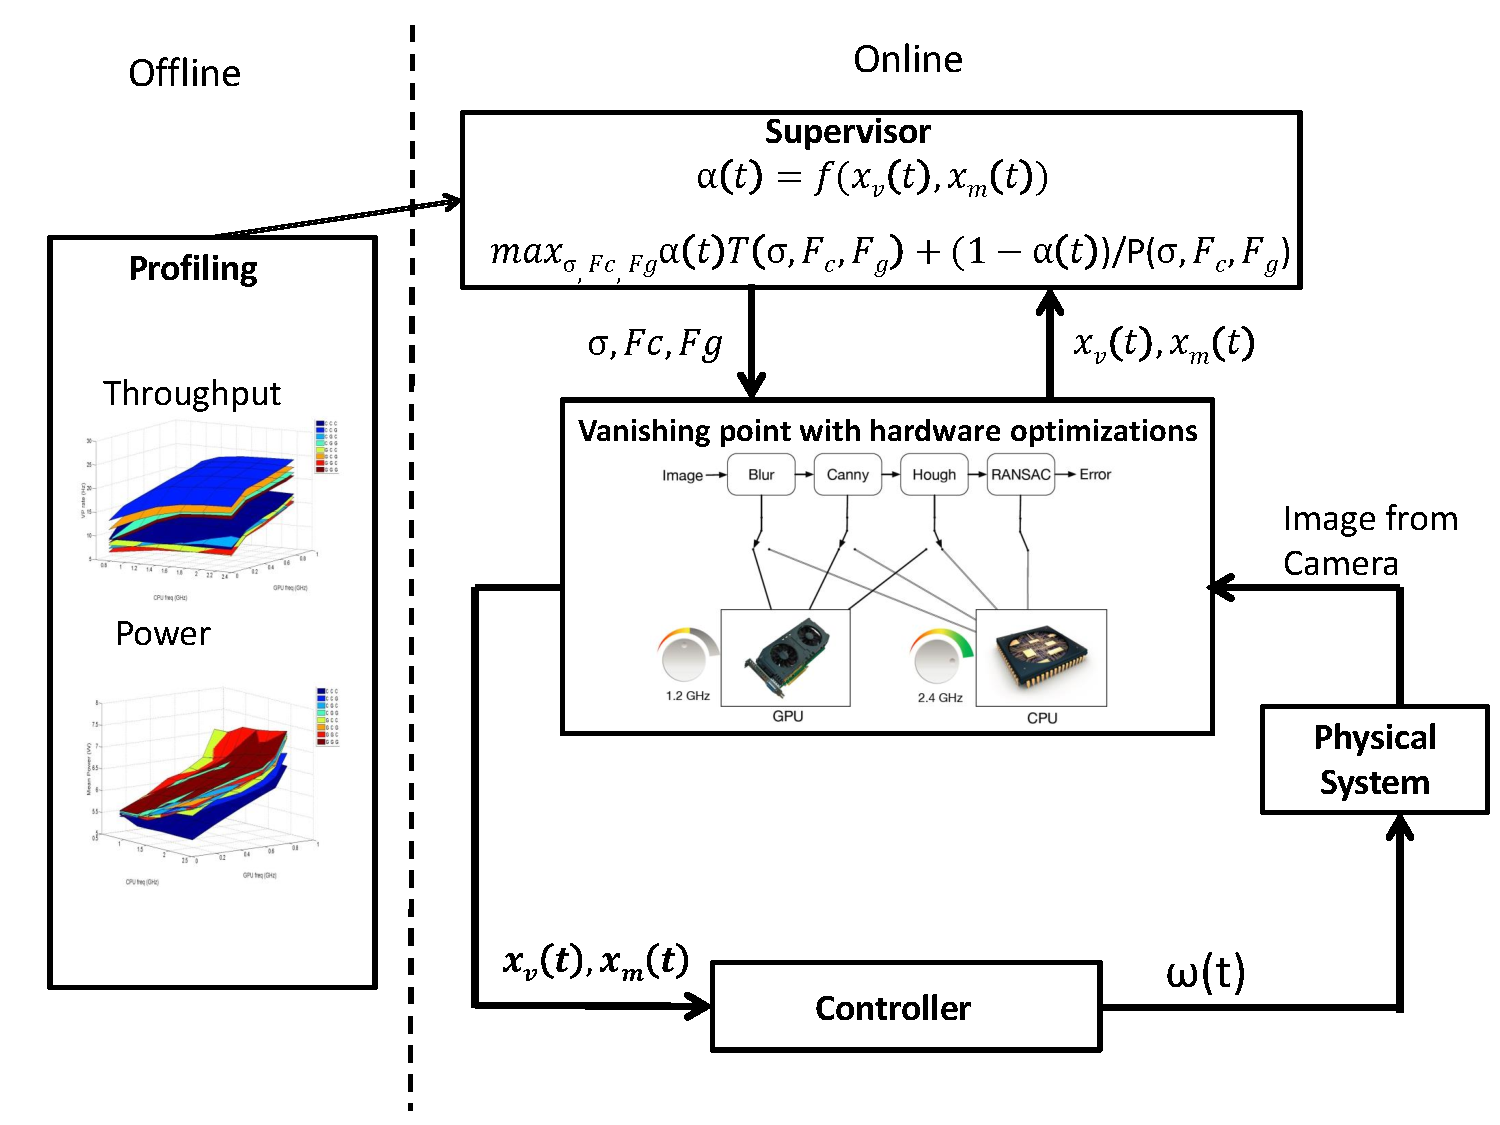
\includegraphics[width=0.46\textwidth]{Figs/bigFig.pdf}
	\caption{Two stage approach.}
	\label{fig:juicyj}%same freq diff assignment}
\end{figure} 


%\section{Experimental setup}

In this work, we focus on the particular case of autonomous corridor navigation. 
For this purpose we use the vanishing point algorithm and PID control to maintain heading parallel to the corridor and stay in the middle of it. We implement our algorithm on a $1/10^{th}$ scale car we developed. This section covers the hardware, the algorithm, and the hardware level knobs which affect the performance of the closed loop system and energy consumption of the computation platform.

\subsection{The hardware}

For our experiments, we converted a Radio controlled Traxxas Rally car into an autonomous robot shown in Fig. \ref{fig:traxxas}, similar to the ones used in \cite{racecar_mit}.

The computation platform is a NVIDIA Jetson TK1. 
The Jetson has a quad-core ARM Cortex-A15 CPU and a NVIDIA Kepler GPU. 
This setup allows us to schedule tasks on the CPU or GPU while observing the effect of this on power consumption and timing of the algorithm. 
The Jetson runs Ubuntu for Tegra as the operating system, and the algorithms are implemented using ROS \cite{ros}. The control signals for the drive and steer motor on the platform are generated by a Teensy 3.1 microcontroller running a ROS node which converts the continuous output of the control software to a PWM signal that acts as an input to the motor controller on the Traxxas. 
Finally, the vanishing point algorithm implemented in OpenCV \cite{opencv} gets images from a front facing Point Grey Firefly MV camera capable of recording color images at upto a resolution of 752x480 pixels and upto a frame rate of 60 FPS. 

\subsection{Vanishing point-based corridor navigation}

The Vanishing point algorithm \cite{VP1} has been used extensively in indoor settings for navigating corridors autonomously \cite{VP2, VP3} and for outdoor lane detection \cite{gallagher2002ground}. 
The algorithm outputs the horizontal distance of the frame's vanishing point from the center of the frame. 
This distance is used by our car's controller to align the robot with the corridor. 

We focus on the major computational tasks that comprise the vanishing point algorithm, shown in fig. \ref{fig:vanishing}.
They are:

\begin{itemize}
\item Blur: A Gaussian blur is applied on the image for de-noising.
\item Edge detection: We use the Canny Edge detector to find edges in the image.
\item Hough Transform: used to detect straight lines in the image.
\item RANSAC: used to select the parallel straight lines that best describe the sides of the corridor. These lines intersect in the image plane at the Vanishing Point.
\end{itemize}

\begin{figure}
	\centering
	\includegraphics[scale=0.3]{vanishing}
	\caption{The vanishing point algorithm with components running on either CPU or GPU at various frequencies, resulting in different power consumptions.}
	\label{fig:vanishing}		
\end{figure}
\subsection{Exploiting hardware level knobs}
With the vanishing point algorithm, we can execute the Blur, the Edge detection and the Hough transform on either the CPU or the GPU. 
RANSAC runs fast enough to not have a significant impact on the total execution time, so we do not consider running it on the GPU.
Execution on the GPU results, in general, in a speed-up over the CPU but at the cost of higher power draw from the Jetson. 
Additionally, on the Jetson, we can control the performance of the CPU and GPU by changing the clock frequencies at which they operate. 
This gives us multi-dimensional knobs on the hardware level that we can control to trade-off computation speed and power consumption.





%\section{Profiling performance and power consumption}
\label{sec:profiling}
For the perception algorithm, the first stage of our method is profiling the performance (timing and, if available, quality) and power consumption of the computation. 
To do this profiling, we first navigate the robot manually in corridors and log video from the on-board camera at a high frame-rate. 
We run Vanishing point on this video offline and profile it with different scheduling of the three components (Blur, Canny and Hough) on the CPU and GPU, and at different frequencies of both processors (Fig. \ref{fig:vanishing}).

We wrote a custom C-code library to log power measurements from a Tektronix PWS4205 Programmable DC power supply at 100Hz. 
For this we communicate with the power supply over USB using the USB Test and Measurement Class (USB-TMC) communication protocol. 

%In order to profile the timing performance of the Vanishing point algorithm with different schedules for the three tasks we allocate on either the CPU or the GPU, and the different clock frequencies for the CPU and the GPU, we have a script that runs the vanishing point algorithm for all settings offline and logs the update rate in Hz as well as individual execution times of the components and the power consumption. 
Since for an algorithm like Vanishing point there is no well-defined notion of ground truth, we do not have a measure of accuracy of the algorithm. 
Instead, Vanishing point's update rate is used as a performance measure, since with faster updates the controller can apply input signals to the car faster, resulting in better control performance. 


\subsection{Results}

Figures \ref{fig:dfsa}, \ref{fig:sfda} show the profiling results for the update rate of the Vanishing Point algorithm for different CPU-GPU allocations of the 3 tasks and different frequencies of the CPU and the GPU. Note, the CPU can be clocked upto 2.32 GHz (on all 4 cores), while the GPU can be clocked upto 0.852 GHz. We select 6 operating frequencies evenly spaced from the minimum and maximum Jetson CPU and GPU frequencies for both the CPU and the GPU. Also note that in these figures, Note, the 3 alphabet combinations imply the resource allocated to the Blur, Canny and Hough transform tasks respectively, e.g. C G C means that the Blur was on the CPU, Canny on the GPU and the Hough transform no the CPU and so on.


\begin{figure}[hbtp]
\centering
\includegraphics[width=0.46\textwidth]{Data/figs/RateHist.pdf}
\caption{Update rate for different frequencies and a given CPU-GPU assignment. For brevity we only consider 3 CPU and GPU frequencies for this figure, ranging from the minimum and maximum of both the CPU and the GPU. }
\label{fig:dfsa} %diff freq same assignment}
\end{figure}

\begin{figure}[htbp]
	\centering
	\includegraphics[width=0.46\textwidth]{Data/figs/surf_Rate.pdf}
	\caption{Update rate for different CPU-GPU assignments at fixed frequencies.}
	\label{fig:sfda}%same freq diff assignment}
\end{figure}

Figures \ref{fig:dfsa_pow}, \ref{fig:sfda_pow} show the profiling of average power consumed during the computations for the vanishing point over all frames in the video used for the profiling.


\begin{figure}[htbp]
\centering
\includegraphics[width=0.46\textwidth]{Data/figs/PowerHist.pdf}
\caption{Mean Power consumed by the Jetson for different frequencies and a given CPU-GPU assignment.  For brevity we only consider 3 CPU and GPU frequencies for this figure, ranging from the minimum and maximum of both the CPU and the GPU.}
\label{fig:dfsa_pow} %diff freq same assignment}
\end{figure}

\begin{figure}[htbp]
	\centering
	\includegraphics[width=0.46\textwidth]{Data/figs/surf_Power.pdf}
	\caption{Mean Power consumed by the Jetson for different CPU-GPU assignments at fixed frequencies.}
	\label{fig:sfda_pow}%same freq diff assignment}
\end{figure}




%\section{Future work}

Given the profiling information, on-going work is focused on developing a supervisory algorithm that decides at run-time what mode the perception algorithm should operate in based on the closed loop performance of the system. 
We are also developing a model predictive controller that can leverage the time/power/quality trade-off while guaranteeing safe operation of the closed loop system (e.g., respecting constraints on position and velocity). A more experimental approach also being looked at is switching between multiple PID controllers (each tuned to one mode of the estimation algorithm) based on the error signal from the vanishing point algorithm, which is the only feedback in the simple corridor navigation system which was considered in this work.

\section{Problem Setup}
\label{sec:problemSetup}
In this section, we present the setup in which we study the throughput/power trade-off and its effect on control performance. 
Specifically, we developed a $1/10^{th}$ scale autonomous car.
The car runs the Vanishing Point algorithm \cite{VP1,VP2} and a feedback controller to navigate a corridor and stay in its middle.
The computation platform on board the car is a Nvidia Jetson, which has a quad-core ARM CPU and a 192 core Nvidia Tegra GPU.


\subsection{Vanishing point for corridor navigation}
\label{sec:vp}
The Vanishing Point algorithm (VP) \cite{VP1} has been used extensively in indoor settings for navigating corridors autonomously \cite{VP2, VP3} and for outdoor lane detection \cite{gallagher2002ground}.
For each image frame, the algorithm outputs the horizontal distances $x_v$ of the vanishing point and $x_m$ of the middle point from the center of the frame. 
The vanishing point is the intersection point of any two parallel lines in the environment, and the middle point indicates the center of the corridor. 
See Fig. \ref{fig:vp_viz}.
These two measurements are used by the feedback controller to center the robot in the corridor and align it with the walls. 
It does so by driving the abscissa $x_v$ and $x_m$ to zero using the following feedback law for the steering rate $\omega$ \cite{VP2}:
\begin{equation}
\omega = \frac{k_1}{k_1k_3+x_mx_v}(-\frac{k_2v}{k_1}x_v -k_px_m)
\label{eq:controller}
\end{equation}
where $k_p,k_1,k_2,k_3$ are parameters, and the car dynamics are modeled as follows:
\begin{equation}
\dot{x} = v\sin\theta,\; \dot{y} = v\cos\theta, \;\dot{\theta} = \omega 
\end{equation}
where $x$ is the car's horizontal position (referenced to an origin in the middle of the corridor), $y$ is its vertical position, and $\theta$ is the steering angle.
The car's velocity $v$ is fixed.
The VP computation time appears as a delay to this controller. 
In general, less delay means better control performance but larger computation power. 
Our goal is to achieve a trade-off where the control performance is acceptable (robot drives along the middle of the corridor) while the computation energy is minimized. 

\begin{figure}[tb]
	\centering
	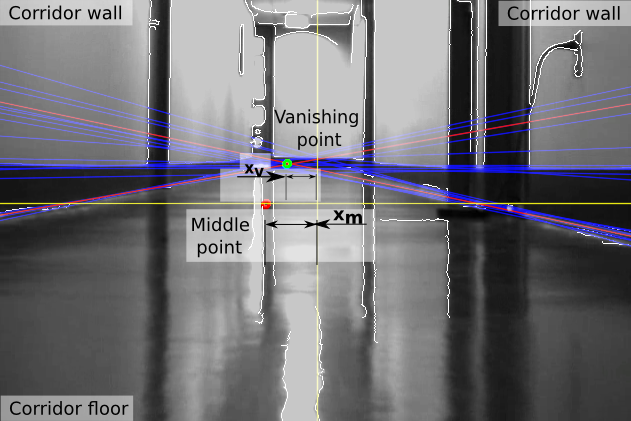
\includegraphics[width=0.49\textwidth]{Figs/vpmpimages/labelled_corridor_4.png}
	\caption{Vanishing point algorithm output overlaid on the corridor image. The green (upper) dot shows the vanishing point while the red (lower) dot shows the middle point. These are computed from the intersection of the detected corridor guidelines. (Color in online version)}
	\label{fig:vp_viz} %diff freq same assignment}
\end{figure}

%\label{sec:robotDynamics}
%In order to simulate the closed loop behaviour of the robot, we use a unicycle model for the dynamic and a non-linear feedback controller as explained in \cite{VP2}. The unicycle dynamics are:
%
%Here, $v$ is the velocity of the robot, which we treat as a constant parameter for our setup. The co-ordinate frame is defined such that $x$ is the distance of the robot from the middle of the corridor. The goal of the closed loop controller is to navigate this robot along the middle of the corridor. Note, the controlled variable is $\omega$, the desired angular velocity of the robot.
%
%With the vanishing point based perception algorithm, the measurements from this system are the vanishing point and middle point abscissas as measured from processing the images from a front facing camera mounted on the robot. Using the geometry of the image frame as explained in \cite{VP2}, these measurements are
%
%\begin{subequations}
%	\begin{align}
%	x_v &= k_1\tan\theta \nonumber \\
%	x_m &= k_2\frac{x}{\cos\theta} + k_3\tan\theta
%	\end{align}
%	\label{eq:measurements}
%\end{subequations}
%
%Note, Eq. \ref{eq:measurements} shows that the vanishing point depends only on the orientation of the robot and the middle point depends on both orientation and position. The objective of our robot is to traverse a corridor while being as close to the middle of the corridor. In order to realize this, we need to bring both $x_v$ and $x_m$ to converge to zero. A non-linear controller based on the non-linear dynamics of the robot (Eq. \ref{eq:plant} and the measurements of $x_v$ and $x_m$ to achieve this is (from \cite{VP2})

%================================================================
 We define \textit{throughput} as the update rate of VP, which is the inverse of its execution time. 
 The faster VP executes, the better the control performance of the closed loop system since the controller sees a small delay. 
 Hence, throughput acts as a proxy for control performance. 
 In most implementations, the perception algorithm is always run at its maximum possible throughput to subject the controller to the smallest possible delays.
 This neglects the power consumed by the computation platform.
 In many autonomous systems, power draw from the computation platform is a significant concern; e.g., in our robot, the Jetson and drive motors are powered by separate energy sources.
 So while we would want to subject the controller to a small delay (operate the perception algorithm at a high throughput), we would also like to minimize the power draw from the computation platform in order to maximize the operating time of the system. 
  

\subsection{Exploiting hardware knobs to trade-off power and throughput}
\label{sec:knobs}
In order to trade-off computation power and throughput of the perception algorithm, we rely on the insight that the GPU can execute some tasks faster than a CPU, albeit at a greater power cost.
Also, executing a task at a higher frequency (on either CPU or GPU) increases throughput, but again at a greater power cost.
Thus, in our setup, we found that running VP on the CPU alone resulted in a low throughput (about 8Hz) and low power consumption (about 5W). 
On the other hand running it on the GPU allowed us to get a throughput in excess of 20Hz, but resulted in a power consumption of over 7W. 
In this section, we describe how to divide VP into tasks and profile VP's performance as we vary the execution frequencies of these tasks and their scheduling on either CPU or GPU.
These tasks are (see Fig. \ref{fig:vanishing}):

\begin{itemize}
\item Blur: A Gaussian blur is applied on the image for de-noising.
\item Edge detection: We use the Canny Edge detector to find edges in the image.
\item Hough Transform: used to detect straight lines in the image.
\item RANSAC: used to select the parallel straight lines that best describe the sides of the corridor. These lines intersect in the image plane at the Vanishing Point.
\end{itemize}

We can schedule any of these tasks to be run on either the CPU or the GPU as shown in Fig. \ref{fig:vanishing}.
Let $\sigma \in \Sigma$ denote a given schedule, where 
\[\Sigma=\{\text{CCC, CCG, CGC, CGG, GCC, GCG, GGC, GGG}\} \]
For example, schedule $\sigma=$ CCG means that the Blur task is done on the CPU, the Edge detection is done on the CPU and the Hough Transform is done the GPU, and so on.
Since RANSAC took a negligible amount of time compared to the other tasks, we always execute it on the CPU.
In addition, we can change the CPU and GPU frequencies during run-time, resulting in different execution times and power consumption for the Jetson. 
Let $F_c$ and $F_g$ be the frequencies of the CPU and the GPU respectively. 

The hardware level knobs to trade-off throughput and computation power for an execution of the vanishing point algorithm are now $\sigma$, $F_c$ and $F_g$. 
The throughput and computation power, functions  of all three knobs, are denoted by $T(\sigma,F_c,F_g)$ and $P(\sigma,F_c,F_g)$ respectively.


\begin{figure}
	\centering
	\includegraphics[scale=0.3]{Figs/vanishing}
	\caption{The vanishing point algorithm with components running on either CPU or GPU at various frequencies, resulting in different power consumptions and execution times.}
	\label{fig:vanishing}		
\end{figure}

\subsection{The Mode Selection problem}
\label{sec:mode selection}
The problem we solve is that of picking the best operating mode ($\sigma$, $F_c$ and $F_g$) for the perception algorithm VP in order to minimize computation power $P(\sigma,F_c,F_g)$ without overly affecting the closed loop control performance of the system, quantified by the throughput $T(\sigma,F_c,F_g)$. 

\section{Two stage approach for hardware optimizations}

\subsection{Offline profiling of performance and power consumption of the perception algorithm}
\label{sec:profiling}
\begin{figure}
	\centering
	\includegraphics[scale=0.3]{Figs/vanishing}
	\caption{The vanishing point algorithm with components running on either CPU or GPU at various frequencies, resulting in different power consumptions and execution times.}
	\label{fig:vanishing}		
\end{figure}

For the perception algorithm, the first stage of our method is profiling the performance (timing and, if available, quality) and power consumption of the computation. With the vanishing point algorithm, we can execute the Blur, the Edge detection and the Hough transform on either the CPU or the GPU (Fig. \ref{fig:vanishing}. RANSAC runs fast enough to not have a significant impact on the total execution time, so we do not consider running it on the GPU. Execution on the GPU results, in general, in a speed-up over the CPU but at the cost of higher power draw from the Jetson. Additionally, on the Jetson, we can control the performance of the CPU and GPU by changing the clock frequencies at which they operate. This gives us multi-dimensional knobs on the hardware level that we can control to trade-off computation speed and power consumption.

To do this profiling offline, we first navigate the robot manually in corridors and log video from the on-board camera at a high frame-rate (60Hz). 
We run Vanishing point algorithm on this video offline and profile it with different scheduling of the three components (Blur, Canny and Hough) on the CPU and GPU, and at different frequencies of both processors.

We wrote a custom C-code library to log power measurements from a Tektronix PWS4205 Programmable DC power supply at 100Hz. 
For this we communicate with the power supply over USB using the USB Test and Measurement Class (USB-TMC) communication protocol. 
 
Since for an algorithm like Vanishing point there is no well-defined notion of ground truth, we do not have a measure of accuracy of the algorithm. 
Instead, Vanishing point's update rate (which is the inverse of the computation time) is used as a performance measure, since with faster updates the controller has less delay, resulting in better control performance. 

\subsubsection{Experimental results for profiling}
%profilingresults


Figure \ref{fig:dfsa} shows the profiling results for the throughput (update rate) of the Vanishing Point algorithm for different CPU-GPU allocations of the 3 tasks and different frequencies of the CPU and the GPU. 
Note, the CPU can be clocked upto 2.32 GHz (on all 4 cores), while the GPU can be clocked upto 0.852 GHz. 
We select 6 operating frequencies evenly spaced from the minimum and maximum Jetson CPU and GPU frequencies for both the CPU and the GPU. 
In these figures, the 3 letter combinations encode the CPU-GPU allocation .
For example, C G C means that the Blur was run on the CPU, Canny on the GPU and the Hough transform on the CPU.


\begin{figure}[htbp]
	\centering
	\includegraphics[width=0.46\textwidth]{Figs/surf_Rate.pdf}
	\caption{Vanishing point algorithm update rate for different CPU-GPU assignments at varying frequencies (color in online version).}
	\label{fig:sfda}%same freq diff assignment}
\end{figure}

%\begin{figure}[hbtp]
%\centering
%\includegraphics[scale=0.3]{Figs/RateHist.pdf}
%\caption{Control update rate for different frequencies and a given CPU-GPU assignment. For clarity we only consider 3 CPU and GPU frequencies for this %figure, ranging from the minimum to the maximum of frequencies of CPU and GPU. (Color in online version) }
%\label{fig:dfsa} %diff freq same assignment}
%\end{figure}

Figure \ref{fig:sfda_pow} showS the profiling of average power consumed during the computations for the vanishing point over all frames in the video used for the profiling.


\begin{figure}[htbp]
	\centering
	\includegraphics[width=0.46\textwidth]{Figs/surf_Power.pdf}
	\caption{Mean power consumed by the Jetson for different CPU-GPU assignments at varying frequencies. (Color in online version)}
	\label{fig:sfda_pow}%same freq diff assignment}
\end{figure}

%\begin{figure}[htbp]
%\centering
%\includegraphics[width=0.46\textwidth]{Figs/PowerHist.pdf}
%\caption{Mean power consumed by the Jetson for different frequencies and a given CPU-GPU assignment.  For clarity we only consider 3 CPU and GPU frequencies for this figure, ranging from the minimum and maximum of both the CPU and the GPU. (Color in online version)}
%\label{fig:dfsa_pow} %diff freq same assignment}
%\end{figure}


\subsection{Feedback driven online scheduling and hardware mode selection}
\label{sec:scheduling}

The profiling results indicate that the knobs $\sigma, F_c$ and $F_g$ allow us to trade-off throughput for power, as expected.
At runtime, we must decide which knob setting to choose at every time step. 
This is done by maximizing the following objective function at every time step $t$:

\begin{equation}
\max_{\sigma,F_{c},F_{g}} \alpha(x_m,x_v)\mathbf{\bar{T}}(\sigma,F_{c},F_{g}) + \frac{1-\alpha(x_m,x_v)}{\mathbf{E[\bar{P}]}(\sigma,F_{c},F_{g})}
\label{eq:cost_runtime}
\end{equation}

Recall that $\mathbf{\bar{T}}(\sigma,F_{c},F_{g})$ is the normalized throughput of VP, and $\mathbf{E[\bar{P}]}(\sigma,F_{c},F_{g})$ is the mean normalized power consumed by the computation platform.
The parameter $\alpha(x_m,x_v) \in [0,1]$ determines how much to weigh throughput versus performance at every time step. 
It is computed as a function of the abscissa $x_m,x_v$: recall that non-zero values of either indicates deviation from the center line of the corridor (Section \ref{sec:vp}). 
Since $x_m,x_v$ are time-varying, $\alpha$ is also time-varying.
As $x_m$ or $x_v$ deviates further away from 0, $\alpha$ increases to more heavily weigh throughput, thus skewing the optimization towards larger throughput and better control performance.
This translates as different CPU-GPU schedules and different frequencies.
In this paper, we use three different functions for $\alpha$, given $d >0$:

{\footnotesize{
		\begin{equation}
		\alpha= f_1(x_v(t)) = \\
		\begin{cases}
		0.001,&\text{if }x_v(t)\in[-d,d]\\
		x_v(t)+d,&\text{if }x_v(t)<-d\\
		x_v(t)-d,&\text{if }x_v(t)>d
		\end{cases}
		\label{eq:f1}
		\end{equation}
	}}
	
	{\footnotesize{
			\begin{equation}
			\alpha = f_2(x_m(t)) = \\
			\begin{cases}
			0.001,&\text{if }x_m(t)\in[-d,d]\\
			x_m(t)+d,&\text{if }x_m(t)<-d\\
			x_m(t)-d,&\text{if }x_m(t)>d
			\end{cases}
			\label{eq:f2}
			\end{equation}
		}}
		
{\footnotesize{
		\begin{equation}
		\alpha = f_3(x_m(t),x_v(t)) \\
		\begin{cases}
		0.001,\text{if }|x_m(t)|+|x_v(t)|<d\\
		|x_m(t)|+|x_v(t)|-d,\text{otherwise}\\
		\end{cases}
		\label{eq:f3}
		\end{equation}
	}}

\section{Simulations}
\label{sec:simulations}

In order to evaluate our approach, we implemented our algorithm in MATLAB and simulated it with two plant models, including the example of Section ??. The set computations were done using the MPT Toolbox ??, and the invariant set computations using the Matlab Invariant Set Toolbox ??. For the reachability computations of Section ??, we perform reachability on the feedback linearized system with MPT using the steps outlined in Section ??, but with $E$ replaced by $\tilde{E}_{max}$ and the control set $U$ replaced by $\oa{V}_{k+j|k}$. The set $\oaXset{k+j}{k}$ is then obtained by applying the diffeomorphism to the set $\oa{Z}_{k+j|k}$, and the properties of Lemma ?? still hold. The RMPC algorithm was implemented in CVX [??] and Gurobi [??] was used as the solver.

\subsection{Toy example}

For the running example of Eq. ??, we show the state trajectories for the feedback linearized system in Fig. ?? and for the non-linear system in Fig ??. The input for the feedback linearized system is shown in Fig. along with its upper and lower rectangular bounds computed online, denoted as $ V^{max}_{k|k}$ and $ V^{min}_{k|k}$ respectively, which make up the input constraint set at time $k$, $V_{k|k}$. Also shown is the global inner approximation for the input $v$. It is worth noting that the bounds computed online allow for much more control action than the conservative $V_{inner-global}$. Fig. ?? shows the input to the actual system, $u$. Note, that $u_k \in U \forall k$, as the defintion for $V_{k|k}$ implies. These figures show that, as formulated, the algorithm stabilizes the system while robustly satisfying the state and input constraints.

\subsection{Single link flexible joint manipulator}

As a more complex example, we consider the single link flexible manipulator dynamics, which have also been covered in ??,??,??. The non-linear plant dynamics are given as:

\begin{equation}
\begin{bmatrix} \dot{x}_1 \\ \dot{x}_2 \\ \dot{x}_3 \\ \dot{x}_4    \end{bmatrix} = \begin{bmatrix} x_2 \\ -\frac{mgl}{I}sin(x_1) - \frac{k}{I}(x_1-x_3)  \\ x_4 \\ \frac{k}{J}(x_1-x_3)  \end{bmatrix} + \begin{bmatrix} 0 \\ 0 \\ 0 \\ \frac{1}{J} \end{bmatrix}u
\end{equation}

This models a system where a motor, with an angular moment of inertia $J$,  is coupled to a uniform thin bar of of mass $m$, length $l$ and moment of inertia $I$, through a flexible link, where the flexibility is modeled by a torsional string with stiffness $k$. Here, $x_2$ is the angle of the motor shaft and $x_4$ the rate. The angle of the bar at the end of the flexible link is $x_1$ and its rate  is $x_3$. The input to the system is the motor torque, given by $u$. 

Without getting into the details of the feedback linearization, the diffeomorphism mapping the states of the non-linear system to the feedback linearized system, which is valid in the domain $x \in \mathbb{R}^4$ is given by:

\begin{equation}
z = T(x) = \begin{bmatrix} x_1 \\ x_2 \\ -\frac{mgl}{I}sin(x_1) -\frac{k}{I}(x_1-x_3) \\ \frac{mgl}{I}x_2cos(x_1) - \frac{k}{I}(x_2-x_4)   \end{bmatrix}
\end{equation}

For the linearization of Eq. ??, where $\hat{z}_k = z_k + M(x_k)e_k$, the matrix $M(x_k)$ is given by:
\begin{equation}
M(x_k) = \begin{bmatrix} 1&0&0&0 \\ 0&1&0&0 \\ -\frac{mgl}{I} cos(x_{1k}) -\frac{k}{I} &0 &\frac{k}{I} &0 \\ \frac{mgl}{I}x_{2k}sin(x_{1k}) & -\frac{mgl}{I} cos(x_{1k}) - \frac{k}{I} & 0 & \frac{k}{I}     \end{bmatrix}
\end{equation}

Also, the input to the feedback linearized system is given by:

\begin{subequations}
\label{eq:fblin_inp}
\begin{align}
v&=\beta u+ \alpha(x) \\
&\text{Where,} \nonumber \\
\beta&=\frac{k}{IJ} \\
\alpha(x)&=\frac{mgl}{I}x_2^2sin(x_1) + \frac{k^2}{IJ}(x_1-x_3) \nonumber \\
&- (\frac{mgl}{I}cos(x_1)-\frac{k}{I})(\frac{mgl}{I}sin(x_1)+\frac{k}{I}(x_1-x_3))
\end{align}
\end{subequations}

The safe set for the states is defined as follows, 
\begin{equation}
 -\begin{bmatrix} \pi/4  \\ \pi/4  \\ \pi \\ \pi \end{bmatrix} \leq x \leq \begin{bmatrix} \pi/4  \\ \pi/4  \\ \pi \\ \pi \end{bmatrix}
\end{equation}

Where the angles and their derivatives are in radians and radians per second respectively. Note, the safe set places a smaller degree of freedom on the range and angular velocities of the rod compared to the motor shaft.
The limits on the input torque, in $Nm$, $u$, are given by the set $U = u :-10 \leq u \leq 10$. The estimation for the state estimation, where $\hat{x} = x + e$ are given by $E = e:-\pi /180 \leq e \leq \pi /180 $, where the units are radians and radians per second accordingly. 

From Eq. \ref{eq:fblin_inp}, we can compute $V_{inner-global} =v: max_{x\in X}\alpha(x) + \beta \underline{u} \leq v \leq min_{x\in X}\alpha(x) + \beta \overline{u}$. Since $X$ is a hyper rectangle, we can compute $\overline{\alpha}(x)_{X} \geq  max_{x\in X}\alpha(x)$ using interval arithmetic, and similarly $\underline{\alpha}(x)_{X} \leq  min_{x\in X}\alpha(x)$, and hence compute (an under-approximation of) $V_{inner-global}$. Here $\underline{u}=-10$ and $\overline{u}=10$ , the upper and lower limits on $u$ that define the set $U$.
Similarly for the input set underapproximation (Eq.??) computed online, we have $\underline{V}_{k+j|k} = v:   max_{x\in \oa{X}_{k+j|k}} \alpha(x) + \beta \underline{u} \leq v \leq  min_{x\in \oa{X}_{k+j|k}}\alpha(x) + \beta \overline{u}$. This set (an under-approximation of it) can also be computed online using interval arithmetic by over-approximating $\oa{x}_{k+j|k}$ by a hyper-rectangle. 

The set of states for the feedback linearized system $Z$ (as computed by ??) is given by:

\begin{equation}
 -\begin{bmatrix} 0.5121  \\ 0.5121  \\ 2.5347 \\ 2.5603 \end{bmatrix} \leq z \leq \begin{bmatrix} 0.5121  \\ 0.5121  \\ 2.5347 \\ 2.5603 \end{bmatrix}
\end{equation}
\section{Experiments}
\label{sec:simResults}

We simulate the system shown in Fig. \ref{fig:juicyj}, where the car is modeled by the dynamics of Eq. \eqref{eq:cardynamics}, the controller is given by Eq. \eqref{eq:controller}, and the supervisor optimizes Eq. \ref{eq:cost_runtime} as explained in Section \ref{sec:evaluation}. 
The controller experiences a delay when receiving update values of $x_m$ and $x_v$. 
This is the computation delay computed offline during the profiling stage. 
The simulation is repeated three times: once for each choice of $\alpha$ from Eqs. \eqref{eq:f1}, \eqref{eq:f2} and \eqref{eq:f3}.
We also simulate two more scenarios: one where the schedule and frequencies are fixed at the highest throughput (highest power) values, and one where they are fixed at the lowest throughput (lowest power) values.

We initialize the robot aligned to the corridor $\theta=0$ but off from the center by 0.25m, i.e. $x=0.25$. 
The controller attempts to bring the robot to the middle of the corridor and align it with the corridor while the supervisor decides the hardware operating mode ($\sigma,F_c,F_g$) as per Sec. \ref{sec:scheduling}. 
At 10 seconds, we apply a steering disturbance to the system, which is a pulse of magnitude 3 degrees per second and a duration of 2 seconds. 
The controller again tries to recover from this disturbance while the supervisor picks the best operating mode for the perception algorithm. 
The closed loop control performance can be measured over a simulation time of $T$ seconds as $L = \int_0^T |x(t)|dt$, 
and the expected energy consumed can be calculated by integrating the expected power based on the selected operating mode. 
Figs. \ref{fig:cpuf} and \ref{fig:gpuf} show the selected CPU and GPU frequency versus time respectively. 
Fig. \ref{fig:power} show the computation power vs time, while Fig. \ref{fig:schedule} shows the schedule $\sigma$ of CPU-GPU allocation for tasks.

Fig. \ref{fig:xvst} shows the trajectory of $x$ versus time.  
It is worth noting that only the trajectory of $x$ for the lowest power, or highest delay mode differs significantly enough from the others so as to be different visually in this plot.


\begin{figure}[t]
\centering
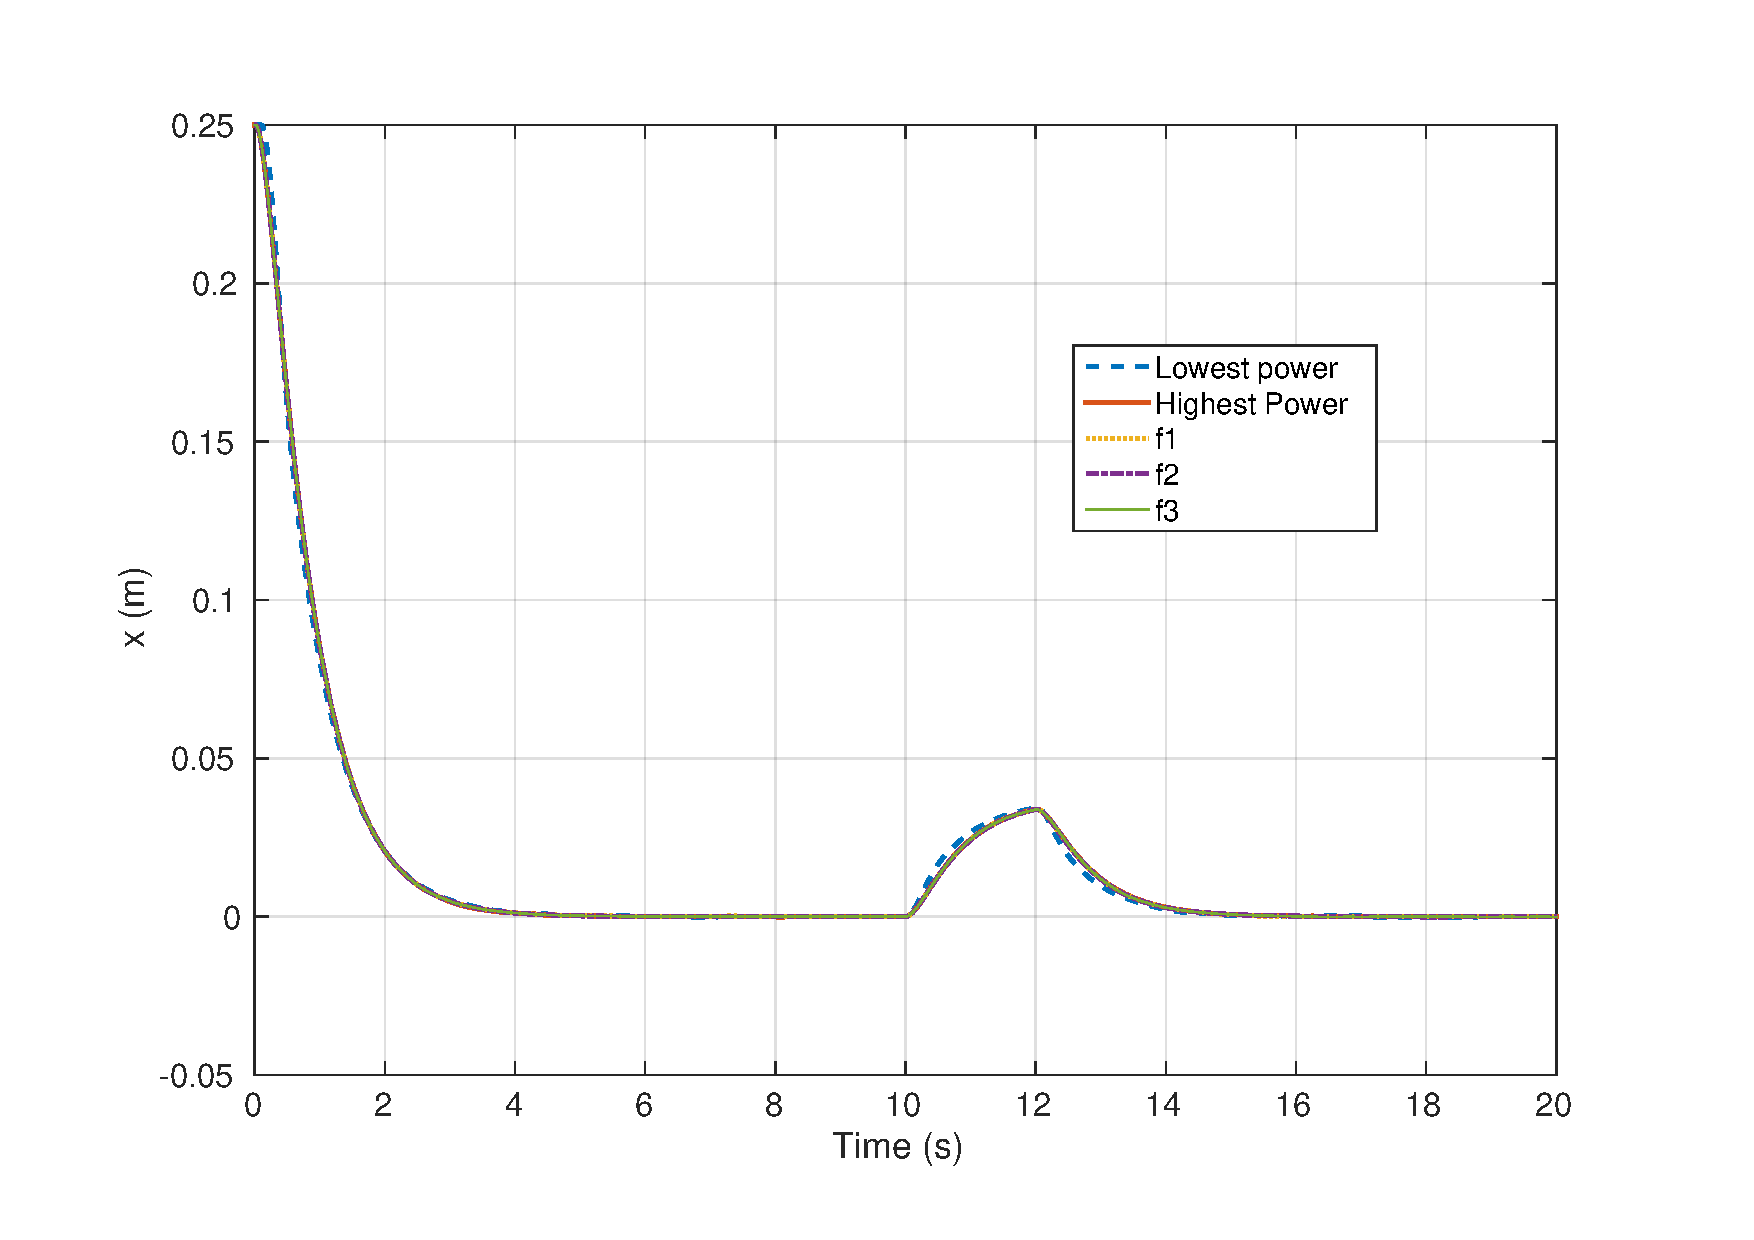
\includegraphics[width=0.49\textwidth]{../simulations/figs/xvst.pdf}
\vspace{-20pt}
\caption{$x$ position of the robot. Note, for modes other than the lowest power (most delay), the trajectory of x is very similar. This is also shown in table \ref{tbl:performance}}.
\label{fig:xvst} 
\end{figure}



To better understand these figures, let us go through 5 checkpoints (\textbf{a}, \textbf{b},\textbf{c}, \textbf{d} and \textbf{e}) in time common to Figs. \ref{fig:xvst}, \ref{fig:cpuf}, \ref{fig:gpuf}, \ref{fig:schedule} ,\ref{fig:power}.
At checkpoint \textbf{a} the controller starts to stabilize $x$ initial displacement of 0.25m. At this time, both $x_v$ and $x_m$ have high magnitudes, implying $\alpha$ takes a high value (close to 1) for all $f_i,\text{ }i=1,2,3$. Due to this, fig. \ref{fig:schedule} shows that $\sigma$ becomes $CCG$ and Figs. \ref{fig:cpuf} and \ref{fig:gpuf} show that CPU and GPU frequencies are high, this implies the vanishing point algorithm is near its highest throughput. Correspondingly, Fig. \ref{fig:power} shows that the computation power is also high.

At checkpoint \textbf{b} $x$ has a small magnitude and is near settling the middle of the corridor. Because of this, both $x_v$ and $x_m$ have smaller magnitudes, and so $\alpha$ is small and the requested CPU and GPU frequencies start to decrease. $\sigma$ is still $CCG$ for all supervisory functions except $f_2$, but settles to $CCC$ for all 3 as $x$ settles to zero shortly after checkpoint \textbf{b}.

Checkpoints \textbf{c}, \textbf{d}, and \textbf{e} show how the system responds to a pulse like disturbance in the steering (lasting from 10s to 12s) and settles (centers and aligns to the corridor) afterwards. It is interesting to see how the different supervisory functions $f_i$ result in different switching between schedule $\sigma=CCC$ and $\sigma=CCG$ and different CPU and GPU frequencies.

 
\begin{figure}[t]
\centering
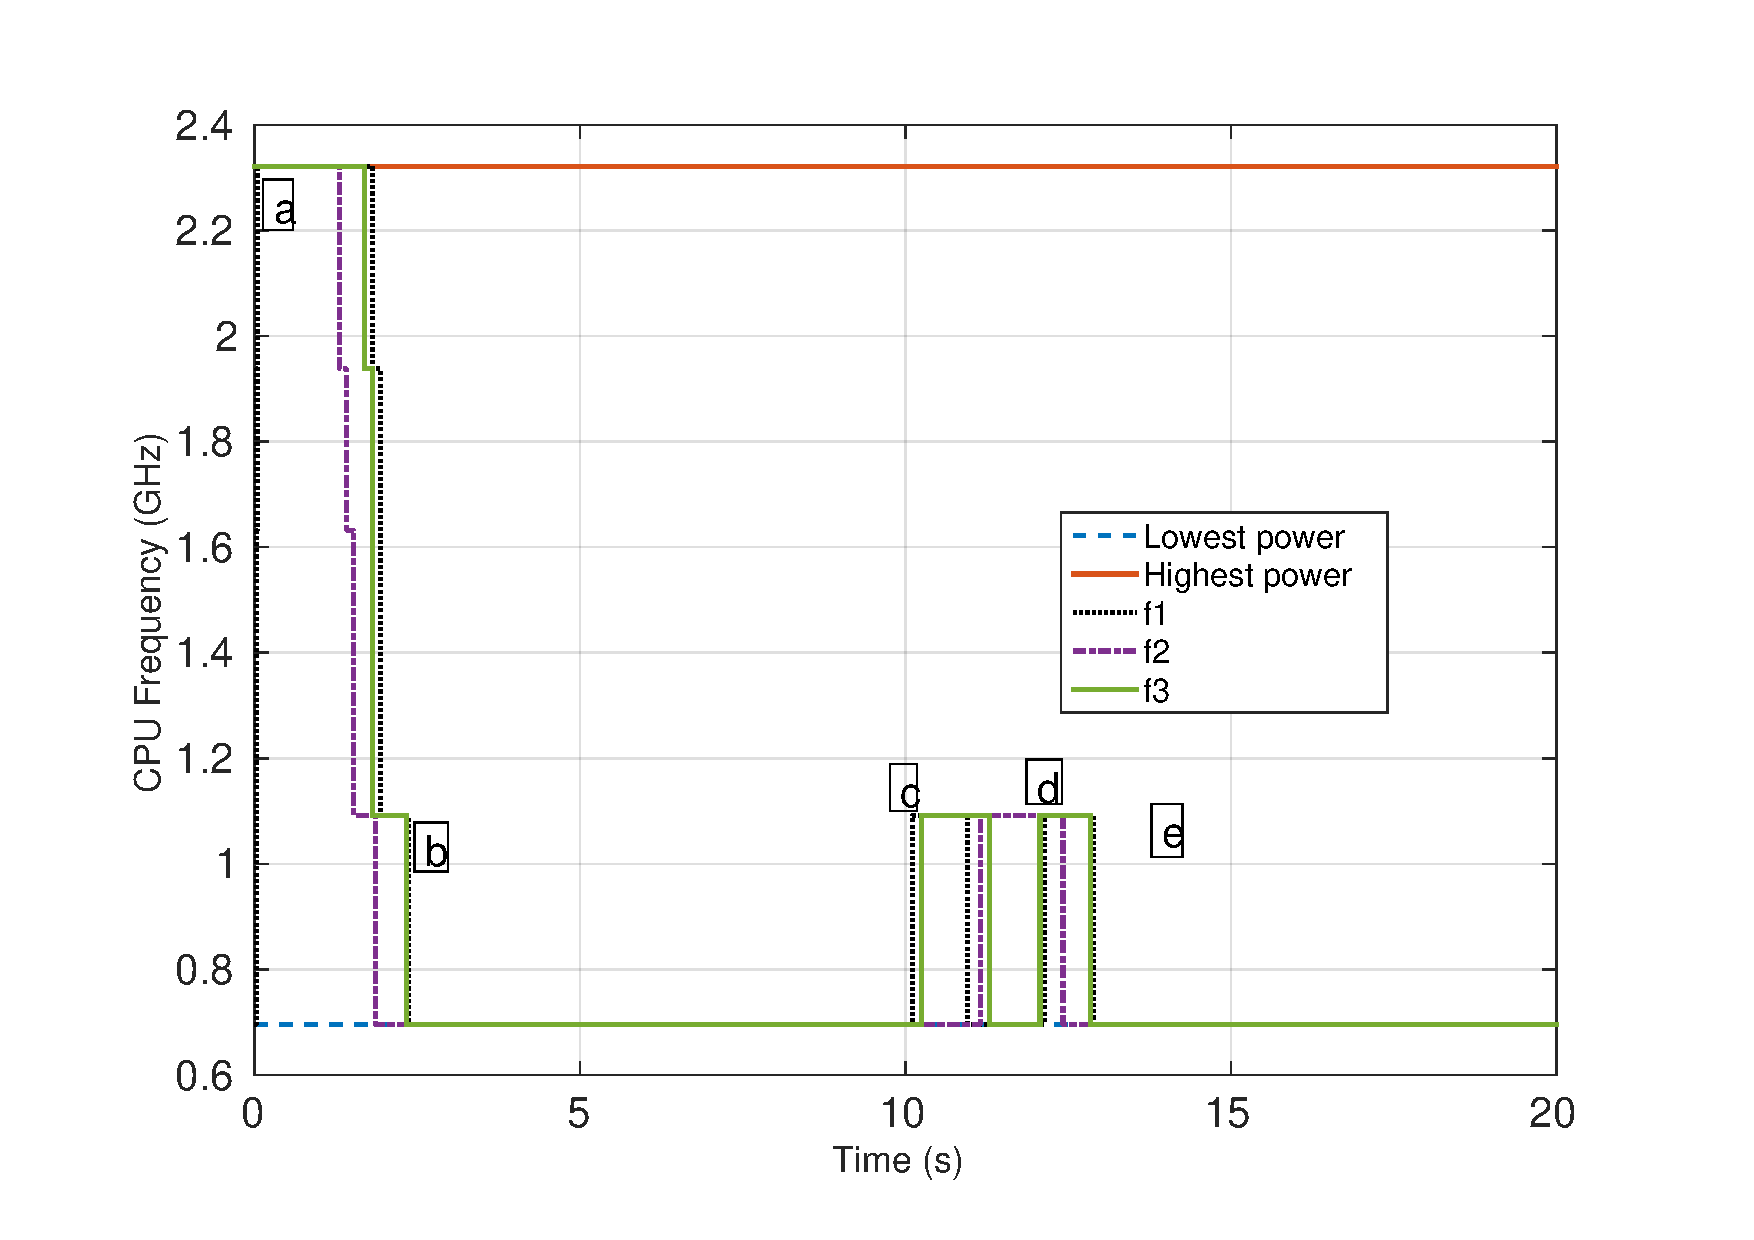
\includegraphics[width=0.49\textwidth]{../simulations/figs/CPUF.pdf}
\vspace{-20pt}
\caption{CPU Frequency selected versus time.}
\label{fig:cpuf} 
\end{figure}


\begin{figure}[t]
\centering
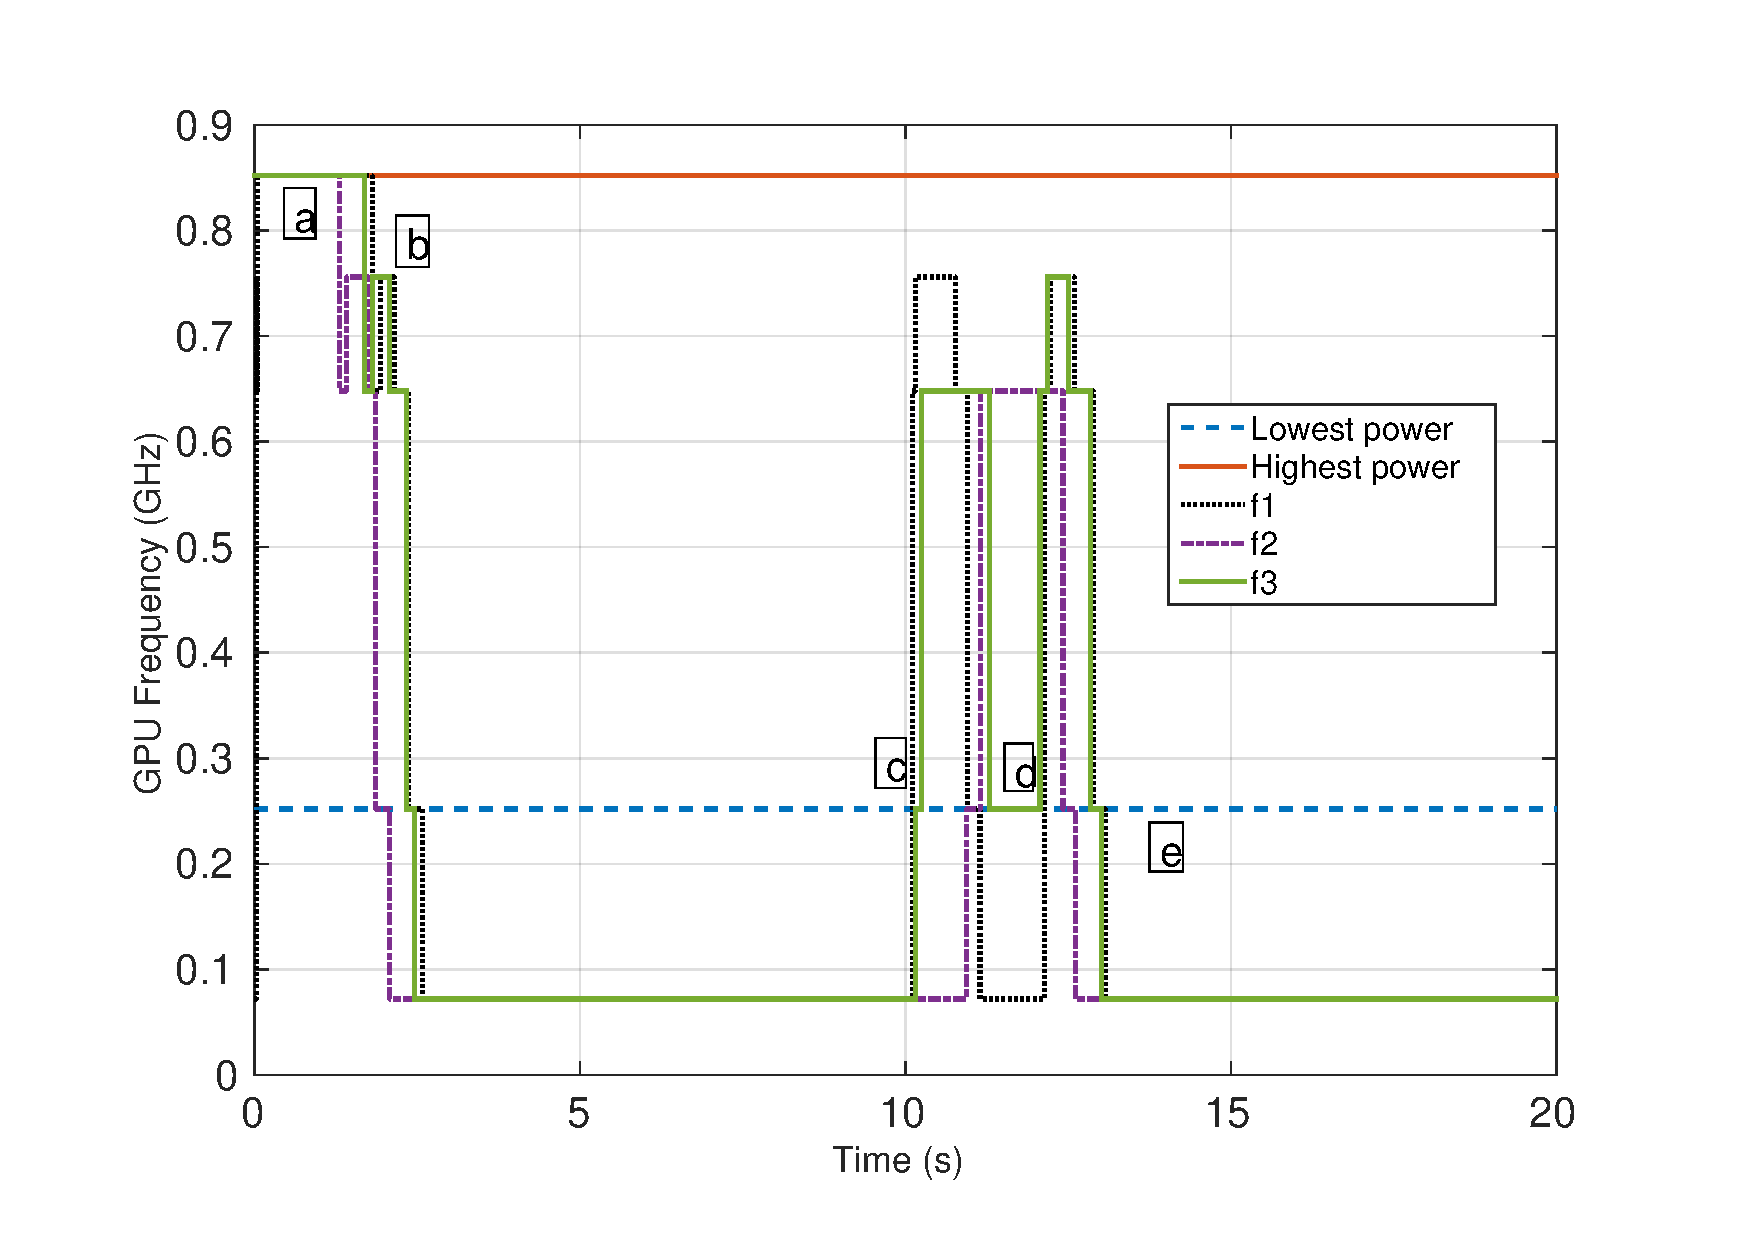
\includegraphics[width=0.49\textwidth]{../simulations/figs/GPUF.pdf}
\vspace{-20pt}
\caption{GPU Frequency selected versus time. Note, for the lowest power mode, the GPU is at its second lowest frequency and not the lowest (while the schedule is $\sigma=CCC$). This is because of the noise in power data while the GPU frequency is being changed while it is not computing any tasks.}
\label{fig:gpuf} 
\end{figure}


\begin{figure}[t]
\centering
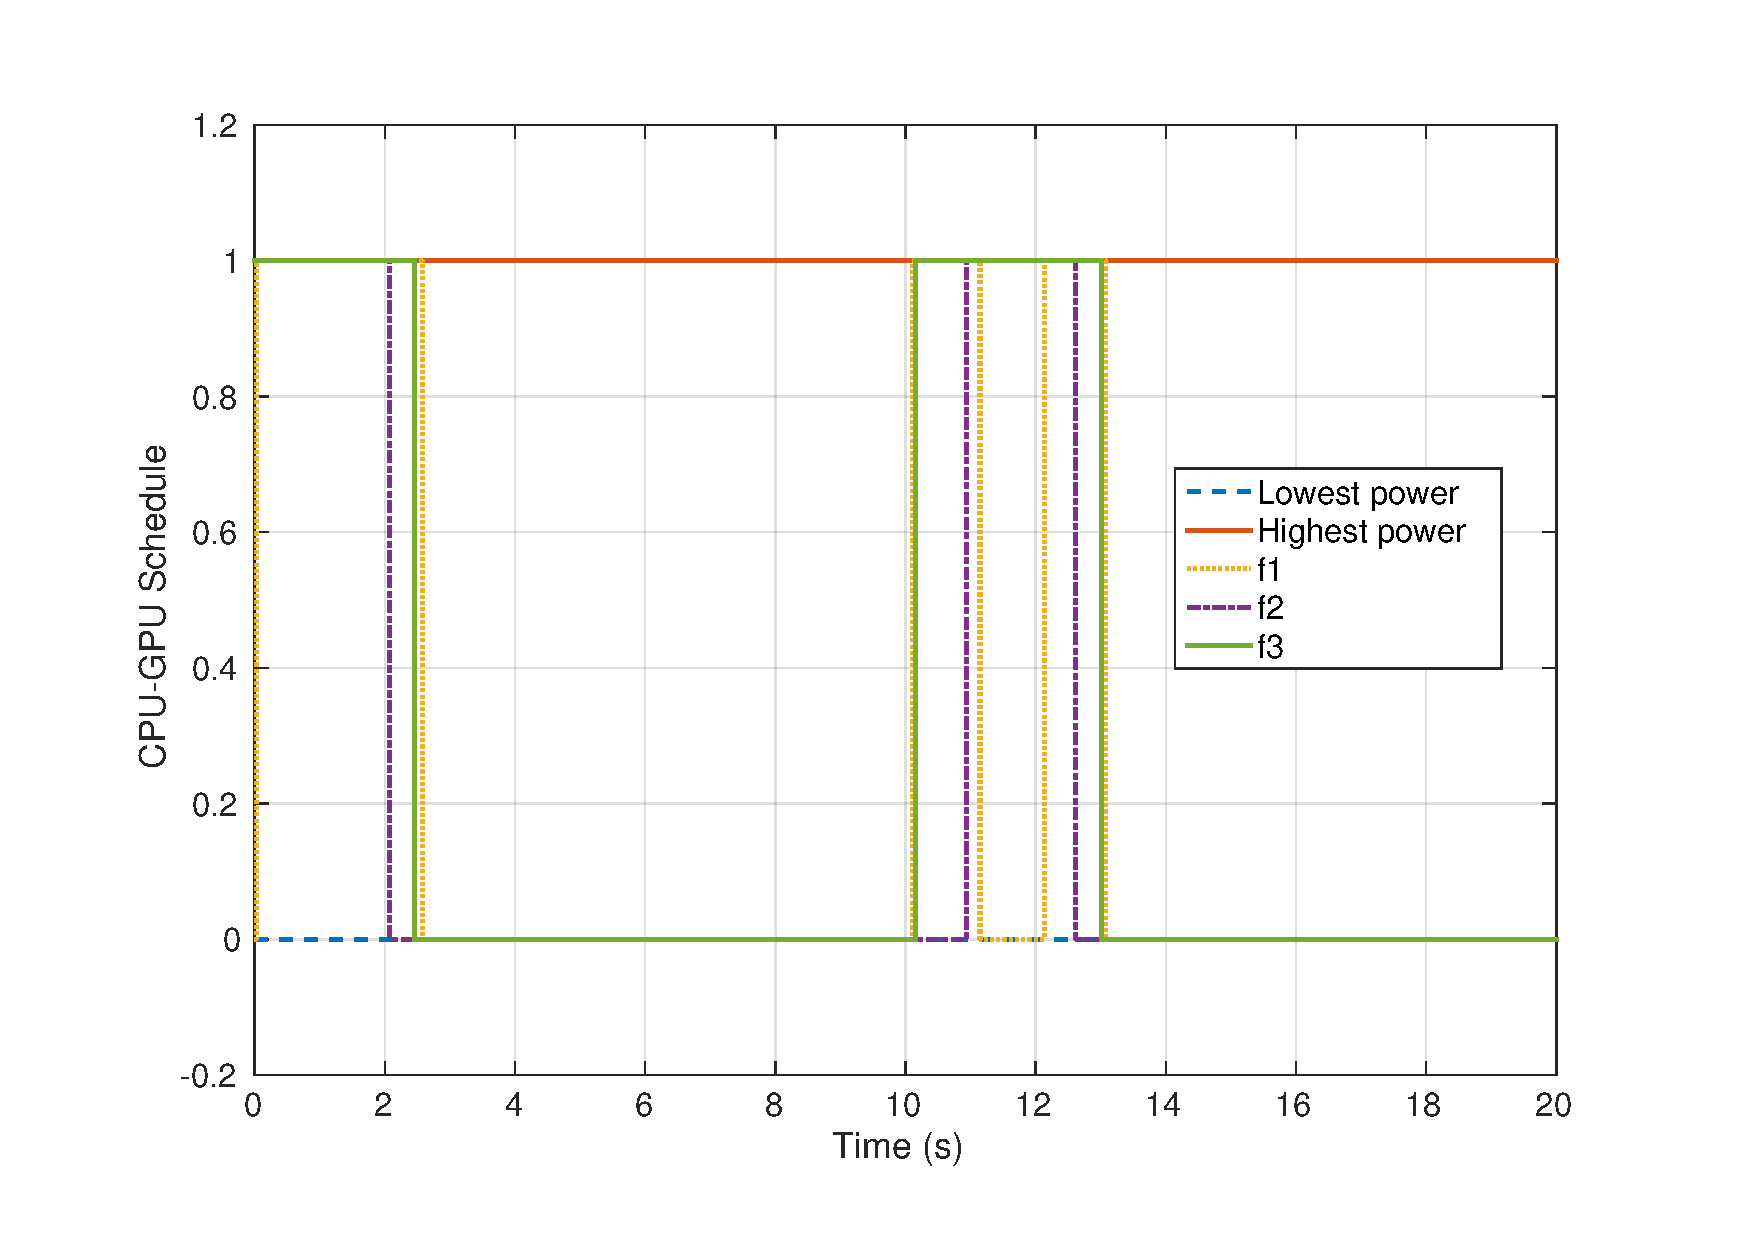
\includegraphics[width=0.49\textwidth]{../simulations/figs/schedule.pdf}
\vspace{-20pt}
\caption{Resource allocation schedule for the vanishing point algorithm. Note, the schedule switches between only two allocations. This is because the allocation $\alpha=CCG$ has the best throughput while having a relatively low power consumption, while $\alpha=CCC$ has the lowest power consumption. See the results in section \ref{sec:profiling} to get a better idea.}
\label{fig:schedule} 
\end{figure}

\begin{figure}[t]
\centering
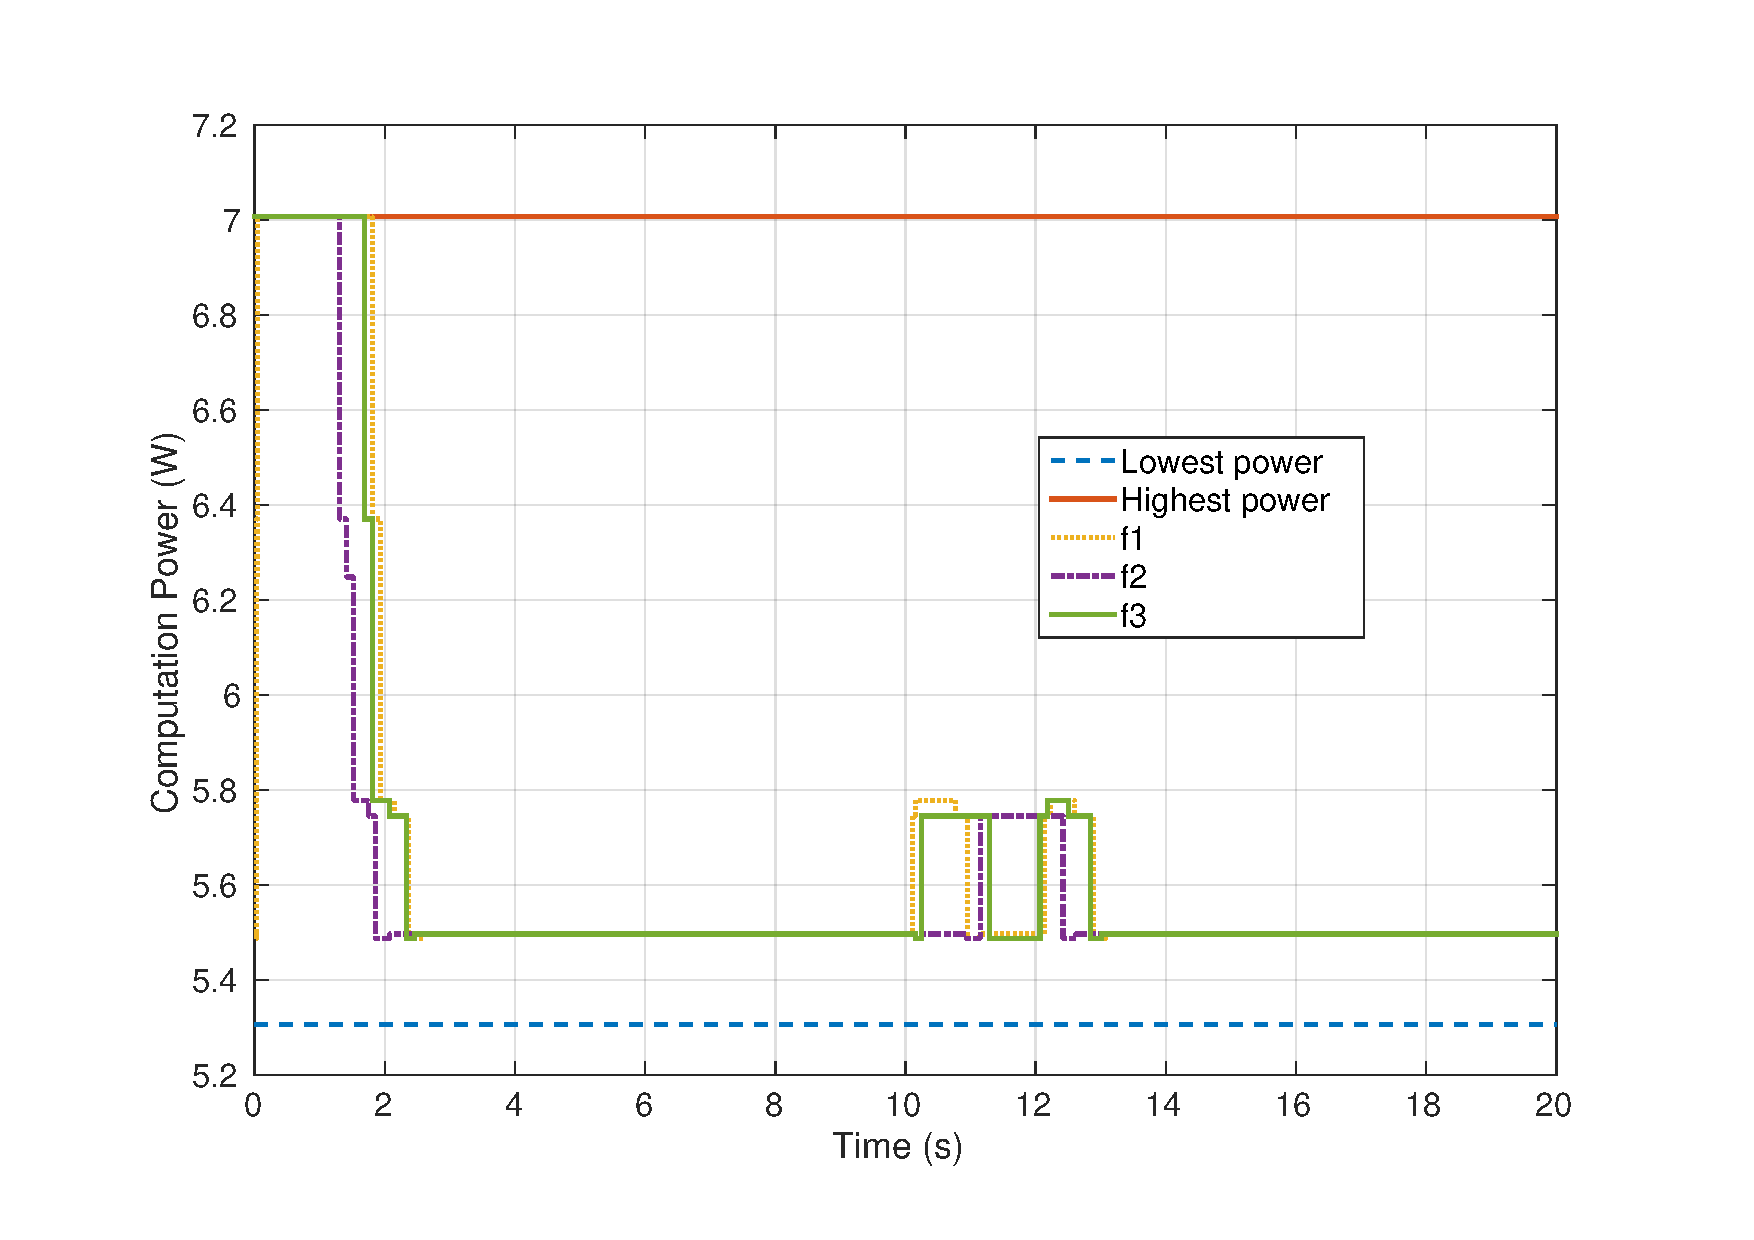
\includegraphics[width=0.49\textwidth]{../simulations/figs/power.pdf}
\vspace{-20pt}
\caption{Average computation power for running VP.}
\label{fig:power} 
\end{figure}

A summary of the control performance and computation energy consumed for these five cases is shown in table \ref{tbl:performance}. It is clear that operating with the highest power/lowest delay mode for the vanishing point results in the best control performance, but the computation energy is high. On the other hand, lowest power/highest delay mode results predictably in low power consumption and the worst control performance. With out two stage approach, control performance is very similar (less than $1\%$ degradation) to the highest power mode, while the computation energy is significantly (about $20\%$) lower. This clearly shows the benefit of our approach.

\begin{table}[htb]
\begin{center}
\caption{Control performance and computation energy}
\label{tbl:performance}
\begin{tabular} {|c|c|c|}
	\hline
	\textbf{Supervisor} & \textbf{Control perf.}(L) & \textbf{Energy}(J) \\ \hline
	Lowest power (mode fixed) & 0.3245 & 106.12  \\ \hline
	Highest power (mode fixed) & 0.3010 & 140.13  \\ \hline
	 $f_1(x_v)$ & 0.3025 & 113.16  \\ \hline
	 $f_2(x_m)$ & 0.3023 & 112.39 \\ \hline
	 $f_3(x_v,x_m)$ & 0.3018 & 113.07 \\ \hline
	 
\end{tabular}
	\vspace{-10pt}	
	\end{center}
\end{table}



\section{Conclusions}
%\todo[inline]{use either formulas or formulae consistently}
%\todo[inline]{use {\small } for figure and table captions}
%\todo[inline]{thre's some funny spacing sometimes..}\todo[inline]{use commas in vectors, [2,2,-1] to distinguish the entries}
%\todo[inline]{we present 3 diff control problems, one with and one without control cost. need to make this a bit smoother, right now it's something of a back and forth between the three. (i know, they're special cases of each other, but it reads bad)}
We present a method to obtain smooth (infinity differentiable) approximations to the robustness of MTL formulae, with bounded and asymptotically decaying approximation error. 
Empirically, we show that the approximation is indeed small for a variety of commonly used MTL formulae. 
Through several examples, we show how we leverage the smoothness property of the approximation for solving a control (or falsification) problem by maximizing (or minimizing) the robustness, using SQP, an off-the-shelf gradient descent optimization technique. 
We compare our technique (SR-SQP) to two other approaches for robustness maximization for control of two dynamical systems, with state and input constraints, and show how our approach consistently outperforms the other two and can be used for control of dynamical systems to satisfy an MTL specification.

%\begin{figure}[t]
%\centering
%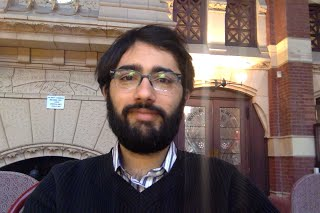
\includegraphics[width=0.49\textwidth]{figures/Habbas}
%\caption{{\small Habbas, pictured here, is the author of this paper, half the papers cited in this paper, half the papers submitted to CPS Week and many others. He can be contacted at habbasATseas.upenn.edu}}
%\label{fig:quad_ssqp}
%\end{figure}

%We would like to thank Kuk Jang for his help in creating diagrams in this paper.
\bibliographystyle{IEEEtran}%abbrv}
	\bibliography{IEEEabrv,rtss2015,cdc14,anytime_ref,rtss_wip_ref}

	%\section*{Appendix}
\label{appendix}

In this appendix we give the detailed mathematical derivation of the results of Section \ctrlProbSecRef.
The controller is designed using a Robust Model Predictive
Control (RMPC) approach via constraint restriction \cite{richardsetal05rmp, chiscietal01swp}, 
and augments it by an adaptation to the error-delay curve of the estimator.
In order to ensure robust safety and feasibility, the key idea of
the RMPC approach is to tighten the constraint sets iteratively to account
for possible effect of the disturbances. 
As time progresses, this ``robustness
margin'' is used in the MPC optimization with the nominal dynamics,
i.e., the original dynamics where the disturbances are either removed
or replaced by nominal disturbances.
%An advantage of this approach is that, 
Because only the nominal dynamics are used, the complexity of the optimization is the same as for the nominal problem.

Since the controller only has access to the estimated state $\hat{x}$, we need
to rewrite the plant's dynamics with respect to $\hat{x}$. 
The error
between $ $$x_{k}$ and $\hat{x}_{k}$ is $e_{k}=x_{k}-\hat{x}_{k}$.
At time step $k+1$ we have
\begin{align*}
\hat{x}_{k+1} & =x_{k+1}-e_{k+1}\\
 & =Ax_{k}+B_{1}(\sDelay_k)u_{k-1}+B_{2}(\sDelay[k])u_{k}+w_{k}-e_{k+1}\text{,}
\end{align*}
 then, by writing $x_{k}=\hat{x}_{k}+e_{k}$, we obtain the dynamics
\begin{equation}
\hat{x}_{k+1}=A\hat{x}_{k}+B_{1}(\sDelay[k])u_{k-1}+B_{2}(\sDelay[k])u_{k}+\hat{w}_{k}\label{eq:estimator-dynamics}
\end{equation}
 where $\hat{w}_{k}=w_{k}+Ae_{k}-e_{k+1}$.
The set of possible values of $\hat{w}_{k}$
depends on the estimation accuracy at steps $k$ and $k+1$ and is
denoted by $\hWc(\sAccu[k],\sAccu[k+1])$, i.e.,
$\hWc(\sAccu,\sAccu')\defeq \left\{ w+Ae-e'\sut w\in\Wc,e\in\ESet(\sAccu),e'\in\ESet(\sAccu')\right\}$.
Note that %we assume
$\hWc(\sAccu[k],\sAccu[k+1])$ is independent
of the time step $k$. %
It can be computed as $\hWc(\sAccu,\sAccu')=\Wc\oplus A\ESet(\sAccu)\oplus\left(-\ESet(\sAccu')\right)$
where the symbol $\oplus$ denotes the Minkowski sum of two sets.

The dynamics in \eqref{eq:estimator-dynamics} has a non-standard form
where it depends on both the current and the previous control inputs.
However we can expand the state variable to store the previous control
input as
\[
\hat{z}_{k}=\begin{bmatrix}\hat{x}_{k}\\
u_{k-1}
\end{bmatrix}\in\Re^{n+m}
\]
and rewrite the dynamics as, for all $k\geq0$,
\begin{equation}
\hat{z}_{k+1}=\hat{A}(\sDelay_k)\hat{z}_{k}+\hat{B}(\sDelay_k)u_{k}+\hat{F}\hat{w}_{k}\text{.}\label{eq:estimator-std-dynamics}
\end{equation}
Here, the system matrices are
\begin{equation}
\begin{gathered}
\hat{A}(\sDelay_k)=\begin{bmatrix}A & B_{1}(\sDelay_k)\\
\bm{0}_{m\times n} & \bm{0}_{m\times m}
\end{bmatrix},\\
\hat{B}(\sDelay_k)=\begin{bmatrix}B_{2}(\sDelay_k)\\
\IdentityMatrix_{m}
\end{bmatrix},\quad\hat{F}=\begin{bmatrix}\IdentityMatrix_{n}\\
\bm{0}_{m\times n}
\end{bmatrix}\text{.}
\end{gathered}
\label{eq:lifted-matrices}
\end{equation}

Let the actual expanded state be $z_{k}=\left[x_{k}^{T},u_{k-1}^{T}\right]^{T}$.
Because the expanded state consists of both the plant's state and
the previous control input, the state constraint $x_{k}\in\stSet$
and the control constraint $u_{k}\in\inpSet$ are equivalent to the
joint constraint $z_{k}\in\stSet\times\inpSet$. We can now describe
the RAMPC algorithm for the dynamics in \eqref{eq:estimator-std-dynamics}.

\subsection{Tractable RAMPC Algorithm}

Let $N\geq1$ be the horizon length of the RMPC optimization. 
Because the system
matrices in the state equation~(\ref{eq:estimator-std-dynamics})
depend nonlinearly on the variables $\sDelay_k$, the RMPC optimization
is generally a mixed-integer nonlinear program, which is very hard
to solve. To simplify the RMPC optimization to make it tractable, we fix the estimation mode for the entire RMPC horizon.

Let $\RAMPCProb{\de}{k}$
denote the RMPC optimization problem at step $k\geq0$ where the current
state estimate is $\hat{x}_{k}$, the current estimation mode is $(\sDelay_k,\sAccu_k)\in\Delta$,
the previous control input is $u_{k-1}$, and the estimation mode
for the entire horizon (after step $k$) is fixed at $(\sDelay,\sAccu)\in\Delta$.
Since the system matrices become constant now, if the stage cost $\ell(\cdot)$
is linear or positive semidefinite quadratic, each optimization problem
$\RAMPCProb{\de}{\cdot}$ is tractable and can be solved
efficiently as we will show later. 
The RAMPC algorithm with Anytime Estimation is stated in Alg. \algoref.

\subsection{RMPC Formulation}

We formulate the RMPC optimization $\RAMPCProb{\de}{k}$
with respect to the nominal dynamics, which is the original dynamics
in \eqref{estimator-std-dynamics} but the disturbances are either
removed or replaced by nominal disturbances. 
To ensure robust feasibility
and safety, the state constraint set is tightened after each step
using a candidate stabilizing state feedback control, and a terminal
constraint is derived. 
In this RMPC formulation, we extend the approach
in \cite{richardsetal05rmp, chiscietal01swp}. 
At time step $k$, given
$(\hat{x}_{k},\sDelay_k,\sAccu_k,u_{k-1})$ and for a fixed $(\sDelay,\sAccu)$,
we solve the following optimization 

\begin{subequations}
	\label{eq:RMPC1}
 \begin{equation} J_{\sDelay,\sAccu}^{*} \left(\hat{x}_{k},\sDelay_k,\sAccu_k,u_{k-1}\right) = \min_{\boldsymbol{u},\boldsymbol{x}}\sum_{j=0}^{N}\ell(\Nom x_{k+j\Given k},u_{k+j\Given k})
 \end{equation}
 \begin{equation}
  \text{subject to, }\forall j\in\left\{ 0,\dots,N\right\} \nonumber 
 \end{equation}
 \begin{equation}
  \Nom z_{k+j+1\Given k}=\hat{A}(\sDelay_{k+j\Given k})\Nom z_{k+j\Given k}+\hat{B}(\sDelay_{k+j\Given k})u_{k+j\Given k}\label{eq:RMPC1-dyn}
 \end{equation}
 \begin{equation}
  ( \sDelay_{k+j+1\Given k},\sAccu_{k+j+1\Given k} ) \!=\! (\sDelay,\sAccu ) \nonumber
 \end{equation}
 \begin{equation}
  (\sDelay_{k\Given k},\sAccu_{k\Given k}) \!=\! (\sDelay_k,\sAccu_k)  \label{eq:RMPC1-delay}
 \end{equation}
 \begin{equation}
  \Nom x_{k+j\Given k}=\begin{bmatrix}\IdentityMatrix_{n} \quad \bm{0}_{n\times m}\end{bmatrix}\Nom z_{k+j\Given k}\label{eq:RMPC1-z2x}
 \end{equation}
 \begin{equation}
  \Nom z_{k\Given k}=\left[\hat{x}_{k}^{T},u_{k-1}^{T}\right]^{T} \label{eq:RMPC1-z0}
 \end{equation}
 \begin{equation}
  \Nom z_{k+j\Given k}\in\ZSet_{j}\left(\sAccu_k,\sAccu\right)\label{eq:RMPC1-zset}
 \end{equation}
 \begin{equation}
  \Nom z_{k+N+1\Given k}\in\ZSet_{f}\left(\sAccu_k,\sAccu\right) \label{eq:RMPC1-zfinalset}
  \end{equation}
\end{subequations} 

in which $\Nom z$ and $\Nom x$
are the variables of the nominal dynamics. The constraints of the
optimization are explained below.
\begin{itemize}
\item \eqref{eq:RMPC1-dyn} is the nominal dynamics.
\item \eqref{eq:RMPC1-delay} states that the estimation mode is fixed at $\left(\sDelay,\sAccu\right)$
except for the first time step when it is $\left(\sDelay_k,\sAccu_k\right)$.
\item \eqref{eq:RMPC1-z2x} extracts the nominal state $\Nom x$ of the plant
from the nominal expanded state $\Nom z$.
\item \eqref{eq:RMPC1-z0} initializes the nominal expanded state at time step
$k$ by stacking the current state estimate and the previous control
input.
\item \eqref{eq:RMPC1-zset} tightens the admissible set of the nominal expanded
states by a sequence of shrinking sets.
\item \eqref{eq:RMPC1-zfinalset} constrains the terminal expanded state to
the terminal constraint set $\ZSet_{f}$.
\end{itemize}

\noindent\textit{The state constraint $\ZSet_{j}$:}
%
The tightened state constraint sets $\ZSet_{j}\left(\sAccu_k,\sAccu\right)$
are parameterized with two parameters $\sAccu_k$ and $\sAccu$.
They are defined as follows, for all $j\in\left\{ 0,\dots,N\right\} $
\begin{eqnarray}
\ZSet_{0}(\sAccu_k,\sAccu)=\ZSet\ominus\hat{F} \ESet(\sAccu_k)\label{eq:RMPC1-Z0}
\\
\ZSet_{j+1}(\sAccu_k,\sAccu)=\ZSet_{j}(\sAccu,\sAccu)\ominus L_{j}\hat{F}\hWc(\sAccu_k,\sAccu)\label{eq:RMPC1-Zj}
\label{eq:RMPC1-Z}
\end{eqnarray} 
in which the symbol $\ominus$
denotes the Pontryagin difference between two sets. The set $\ZSet$
combines the constraints for both the plant's state and the control
input: $\ZSet=\stSet\times\inpSet$. The matrix $L_{j}$ is the state
transition matrix for the nominal dynamics in \eqref{eq:RMPC1-dyn} under
a candidate state feedback gain $K_{j}(\sDelay)$, for $j\in\left\{ 0,\dots,N\right\}$
\begin{eqnarray}
\label{eq:RMPC1-L}
L_{0}=\IdentityMatrix\label{eq:RMPC1-L0}\\
L_{j+1}=(\hat{A}(\sDelay)+\hat{B}(\sDelay)K_{j}(\sDelay))L_{j}\label{eq:RMPC1-Lj}
\end{eqnarray}
Note that the possibly time-varying sequence $K_{j}(\sDelay)$ is designed for each choice of $\sDelay$ (i.e., the system matrices $\hat{A}(\sDelay)$ and $\hat{B}(\sDelay)$), hence $L_{j}$ depends on $\sDelay$; however we write $L_{j}$ for brevity. The candidate control $K_{j}(\sDelay)$ is designed to stabilize the nominal system (\ref{eq:RMPC1-dyn}), desirably as fast as possible so that the sets $\ZSet_{j}$ are shrunk as little as possible. In particular, if $K_{j}(\sDelay)$ renders the nominal system nilpotent after $M<N$ steps then $L_{j}=\bm{0}$ for all $j\geq M$, therefore $\ZSet_{j}\left(\sAccu_k,\sAccu\right)=\ZSet_{M}\left(\sAccu_k,\sAccu\right)$ for all $j>M$.


\noindent\textit{The terminal constraint $\ZSet_{f}$:}
%
$\ZSet_{f}$ is given by %the Pontryagin difference
\begin{equation}
\label{eq:RMPC1-Zf}
\ZSet_{f}\left(\sAccu_k,\sAccu\right)=\Cc(\sDelay,\sAccu)\ominus L_{N}\hat{F}\hWc(\sAccu_k,\sAccu)
\end{equation}
where $\Cc(\sDelay,\sAccu)$ is a robust control invariant admissible
set for $\sDelay$ \cite{kerrigan00rcs}, i.e., there exists a feedback control law $u=\kappa(z)$
such that $\forall z\in\Cc(\sDelay,\sAccu)$ and $\forall w\in\hWc(\sAccu,\sAccu)$
\begin{eqnarray}
\label{eq:RMPC1-Zf-invariant}
& \hat{A}(\sDelay)z \!+\! \hat{B}(\sDelay)\kappa(z) \!+\! L_{N}\hat{F}w\in\Cc(\sDelay,\sAccu) \label{eq:RMPC1-Zf-invariant-dyn}\\
& z\in\ZSet_{N}\left(\sAccu,\sAccu\right)\label{eq:RMPC1-Zf-invariant-z}
\end{eqnarray}
We remark that $\Cc(\sDelay,\sAccu)$ does not depend on $\left(\sDelay_k,\sAccu_k\right)$, therefore it can be computed offline for each mode $\left(\sDelay,\sAccu\right)$.

\subsection{Proofs of Feasibility}
The RMPC formulation of the previous section, with a fixed estimation mode
$\left(\sDelay,\sAccu\right)\in\Delta$, is designed to ensure that the control problem is robustly feasible, as stated in the following theorem.
\begin{thm}
[Robust Feasibility of RAMPC]\label{thm:robust-feasible-RMPC} For
any estimation mode $\left(\sDelay,\sAccu\right)$, if $\RAMPCProb{\de}{k}$
is feasible then the system (\ref{eq:disc-dynamics}) controlled by
the RAMPC and subjected to disturbances constrained by $w_k \in \Wc$
robustly satisfies the state constraint $\stPt_k \in \stSet$
and the control input constraint $\inpPt_k \in \inpSet$, and
all subsequent optimizations $\MPCProb{\sDelay,\sAccu}(\hat{x}_{k},\sDelay[k],\sAccu[k],u_{k-1})$,
$\forall k>k_{0}$, are feasible.
\end{thm}
\begin{proof}
%
We will prove the theorem by recursion. We will show that if at any
time step $k$ the RMPC problem $\MPCProb{\sDelay,\sAccu}(\hat{x}_{k},\sDelay[k],\sAccu[k],u_{k-1})$
is feasible and feasible control input $u_{k}=u_{k\Given k}^{\star}$
is applied with estimation mode $\left(\sDelay[k+1],\sAccu[k+1]\right)=\left(\sDelay,\sAccu\right)$
then $u_{k}$ is admissible and at the next time step $k+1$, the
actual plant's state $x_{k+1}$ is inside $\stSet$ and the optimization
$\MPCProb{\sDelay,\sAccu}(\hat{x}_{k+1},\sDelay[k+1],\sAccu[k+1],u_{k})$
is feasible for all disturbances. Then we can conclude the theorem
because, by recursion, feasibility at time step $k_{0}$ implies robust
constraint satisfaction and feasibility at time step $k_{0}+1$, and
so on at all subsequent time steps.

Suppose $\MPCProb{\sDelay,\sAccu}(\hat{x}_{k},\sDelay[k],\sAccu[k],u_{k-1})$
is feasible. Then it has a feasible solution $\left(\{ \overline{z}_{k+j\Given k}^{\star}\} _{j=0}^{N+1},\{ u_{k+j\Given k}^{\star}\} _{j=0}^{N}\right)$
that satisfies all the constraints in \eqref{eq:RMPC1}. Now we will
construct a feasible candidate solution for $\MPCProb{\sDelay,\sAccu}(\hat{x}_{k+1},\sDelay[k+1],\sAccu[k+1],u_{k})$
at the next time step by shifting the above solution by one step.
Consider the following candidate solution for $\MPCProb{\sDelay,\sAccu}(\hat{x}_{k+1},\sDelay[k+1],\sAccu[k+1],u_{k})$:
\begin{subequations}
\label{eq:proofs:candidate-solution}
\begin{align}
\Nom z_{k+j+1\Given k+1} & =\Nom z_{k+j+1\Given k}^{\star}+L_{j}\hat{F}\hat{w}_{k}\label{eq:proofs:candidate-solution:zj}\\
\Nom z_{k+N+2\Given k+1} & =\hat{A}\left(\sDelay\right)\Nom z_{k+N+1\Given k+1}+\hat{B}\left(\sDelay\right)u_{k+N+1\Given k+1}\label{eq:proofs:candidate-solution:zN}\\
u_{k+i+1\Given k+1} & =u_{k+i+1\Given k}^{\star}+K_{i}\left(\sDelay\right)L_{i}\hat{F}\hat{w}_{k}\label{eq:proofs:candidate-solution:uj}\\
u_{k+N+1\Given k+1} & =\kappa\left(\Nom z_{k+N+1\Given k+1}\right)\label{eq:proofs:candidate-solution:uN}
\end{align}
\end{subequations} in which
$j\in\left\{ 0,\dots,N\right\} $, $i\in\left\{ 0,\dots,N-1\right\} $,
and $\kappa\left(\cdot\right)$ is the feedback control law for the
invariant set $\Cc(\sDelay,\sAccu)$ that is used in the terminal
set. We first show that the input and
state constraints are satisfied for $u_{k}$ and $x_{k+1}$, then
we will prove the feasibility of the above candidate solution for
$\MPCProb{\sDelay,\sAccu}(\hat{x}_{k+1},\sDelay[k+1],\sAccu[k+1],u_{k})$.

\noindent\textit{Validity of the applied input and the next state:}
%
The next plant's state is 
\begin{align*}
x_{k+1} & =Ax_{k}+B_{1}\left(\sDelay[k]\right)u_{k-1}+B_{2}\left(\sDelay[k]\right)u_{k}+w_{k}\\
 & =A\left(\hat{x}_{k}+e_{k}\right)+B_{1}\left(\sDelay[k]\right)u_{k-1}+B_{2}\left(\sDelay[k]\right)u_{k\Given k}^{\star}+w_{k}\\
 & =\begin{bmatrix}A & B_{1}\left(\sDelay[k]\right)\end{bmatrix}\begin{bmatrix}\hat{x}_{k}\\
u_{k-1}
\end{bmatrix}+B_{2}\left(\sDelay[k]\right)u_{k\Given k}^{\star} \\
&\qquad\qquad + e_{k+1}+\left(w_{k}+Ae_{k}-e_{k+1}\right)
\end{align*}
in which $e_{k+1}\in\ESet\left(\sAccu\right)$ and $\left(w_{k}+Ae_{k}-e_{k+1}\right)\in\hWc\left(\sAccu[k],\sAccu\right)$.
Note that $\Nom z_{k\Given k}^{\star}=\left[\hat{x}_{k}^{T},u_{k-1}^{T}\right]^{T}$.
Hence we have
\begin{align*}
\begin{bmatrix}x_{k+1}\\
u_{k}
\end{bmatrix} & =\hat{A}(\sDelay[k])\Nom z_{k\Given k}^{\star}+\hat{B}(\sDelay[k])u_{k\Given k}^{\star}\\
&\qquad\qquad +\hat{F}e_{k+1}+\hat{F}\left(w_{k}+Ae_{k}-e_{k+1}\right)\\
 & =\Nom z_{k+1\Given k}^{\star}+\hat{F}e_{k+1}+\hat{F}\left(w_{k}+Ae_{k}-e_{k+1}\right)
\end{align*}
where we use the dynamics in \eqref{eq:RMPC1-dyn}. From \eqref{eq:RMPC1-zset}
and \eqref{eq:RMPC1-Z}, $\Nom z_{k+1\Given k}^{\star}$ satisfies $\Nom z_{k+1\Given k}^{\star}\in\ZSet_{1}\left(\sAccu[k],\sAccu\right)=\ZSet\ominus\hat{F}\ESet\left(\sAccu\right)\ominus\hat{F}\hWc\left(\sAccu[k],\sAccu\right)$.
It follows that
\(
\left[ x_{k+1}^{T}, u_{k}^{T} \right]^{T} \in \ZSet = \stSet\times\inpSet\text{,}
\)
% which allows us to conclude that
therefore  $x_{k+1}\in\stSet$ and $u_{k}\in\inpSet$.


\noindent\textit{Initial condition:}
%
We have from \eqref{eq:estimator-std-dynamics} that $\hat{z}_{k+1}=\hat{A}(\sDelay[k])\hat{z}_{k}+\hat{B}(\sDelay[k])u_{k}+\hat{F}\hat{w}_{k}$.
On the other hand, by \eqref{eq:proofs:candidate-solution:zj},
\begin{align*}
\Nom z_{k+1\Given k+1} & =\Nom z_{k+1\Given k}^{\star}+L_{0}\hat{F}\hat{w}_{k}\\
 & =\hat{A}(\sDelay[k])\Nom z_{k\Given k}^{\star}+\hat{B}(\sDelay[k])u_{k\Given k}^{\star}+L_{0}\hat{F}\hat{w}_{k}\text{.}
\end{align*}
Note that $\Nom z_{k\Given k}^{\star}=\hat{z}_{k}$, $u_{k}=u_{k\Given k}^{\star}$,
and $L_{0}=\IdentityMatrix$. Therefore $\Nom z_{k+1\Given k+1}=\hat{z}_{k+1}$,
hence the initial condition is satisfied.


\noindent\textit{Dynamics:}
%
We show that the candidate solution satisfies the dynamics constraint
in \eqref{eq:RMPC1-dyn}. For $0\leq j<N$ we have
\begin{align*}
&\Nom z_{k+j+2\Given k+1} \\
=\, & \Nom z_{k+j+2\Given k}^{\star}+L_{j+1}\hat{F}\hat{w}_{k}\\
=\, &\hat{A}\left(\sDelay\right)\Nom z_{k+j+1\Given k}^{\star}+\hat{B}(\sDelay)u_{k+j+1\Given k}^{\star}+L_{j+1}\hat{F}\hat{w}_{k}\\
=\, &\hat{A}\left(\sDelay\right)\left(\Nom z_{k+j+1\Given k+1}-L_{j}\hat{F}\hat{w}_{k}\right) \\
&+\hat{B}(\sDelay)\left(u_{k+j+1\Given k+1}-K_{j}\left(\sDelay\right)L_{j}\hat{F}\hat{w}_{k}\right) +L_{j+1}\hat{F}\hat{w}_{k} \\
=\, &\hat{A}\left(\sDelay\right)\Nom z_{k+j+1\Given k+1}+\hat{B}(\sDelay)u_{k+j+1\Given k+1} \\
&-\left(\hat{A}\left(\sDelay\right) + \hat{B}(\sDelay)K_{j}\left(\sDelay\right)\right)L_{j}\hat{F}\hat{w}_{k}+L_{j+1}\hat{F}\hat{w}_{k}\\
=\, &\hat{A}\left(\sDelay\right)\Nom z_{k+j+1\Given k+1}+\hat{B}(\sDelay)u_{k+j+1\Given k+1}
\end{align*}
where the equality in \eqref{eq:RMPC1-Lj} is used to derive the last
equality. % from the previous one.
Therefore the dynamics constraint
is satisfied for all $0\leq j<N$. For $j=N$, the constraint is satisfied
by construction by \eqref{eq:proofs:candidate-solution:zN}.


\noindent\textit{State constraints:}
%
We need to show that $\Nom z_{(k+1)+j\Given k+1}\in\ZSet_{j}\text{\ensuremath{\left(\sAccu,\sAccu\right)}}$
for all $j\in\left\{ 0,\dots,N\right\} $. Consider any $0\leq j<N$.
\eqref{eq:RMPC1-Zj} states that $\ZSet_{j+1}\left(\sAccu[k],\sAccu\right)=\ZSet_{j}\left(\sAccu,\sAccu\right)\ominus L_{j}\hat{F}\hWc\left(\sAccu[k],\sAccu\right)$.
From the construction of the candidate solution we have $\Nom z_{k+j+1\Given k+1}=\Nom z_{k+j+1\Given k}^{\star}+L_{j}\hat{F}\hat{w}_{k}$,
where $\hat{w}_{k}\in\hWc\left(\sAccu[k],\sAccu\right)$ and $\Nom z_{k+j+1\Given k}^{\star}\in\ZSet_{j+1}\left(\sAccu[k],\sAccu\right)$.
By definition of the Pontryagin difference, we conclude that $\Nom z_{k+j+1\Given k+1}\in\ZSet_{j}\left(\sAccu,\sAccu\right)$
for all $j\in\left\{ 0,\dots,N-1\right\} $.

At $j=N$ the candidate solution in \eqref{eq:proofs:candidate-solution:zj}
gives us $\Nom z_{(k+1)+N\Given k+1}=\Nom z_{k+N+1\Given k}^{\star}+L_{N}\hat{F}\hat{w}_{k}$.
Because $\Nom z_{k+N+1\Given k}^{\star}\in\ZSet_{f}\left(\sAccu[k],\sAccu\right)=\Cc\left(\sDelay,\sAccu\right)\ominus L_{N}\hat{F}\hWc\left(\sAccu[k],\sAccu\right)$
and $\hat{w}_{k}\in\hWc\left(\sAccu[k],\sAccu\right)$, we have
$\Nom z_{(k+1)+N\Given k+1}\in\Cc\left(\sDelay,\sAccu\right)$. The
definition of $\Cc\left(\sDelay,\sAccu\right)$ in \eqref{eq:RMPC1-Zf-invariant}
implies $\Cc\left(\sDelay,\sAccu\right)\subseteq\ZSet_{N}\left(\sAccu,\sAccu\right)$.
Therefore $\Nom z_{(k+1)+N\Given k+1}\in\ZSet_{N}\left(\sAccu,\sAccu\right)$.


\noindent\textit{Terminal constraint:}
%
We need to show that $\Nom z_{k+N+2\Given k+1}\in\ZSet_{f}\left(\sAccu,\sAccu\right)=\Cc\left(\sDelay,\sAccu\right)\ominus L_{N}\hat{F}\hWc\left(\sAccu,\sAccu\right)$.
Add $L_{N}\hat{F}\hat{w}$, for any $w\in\hWc\left(\sAccu,\sAccu\right)$,
to both sides of \eqref{eq:proofs:candidate-solution:zN} and note that
$u_{k+N+1\Given k+1}=\kappa\left(\Nom z_{k+N+1\Given k+1}\right)$,
we have 
\begin{multline*}
  \Nom z_{k+N+2\Given
    k+1}+L_{N}\hat{F}\hat{w}=\hat{A}\left(\sDelay\right)\Nom
  z_{k+N+1\Given k+1} \\
  +\hat{B}\left(\sDelay\right)\kappa\left(\Nom
    z_{k+N+1\Given k+1}\right)+L_{N}\hat{F}\hat{w}\text{.}
\end{multline*}


 It follows from $\Nom z_{k+N+1\Given k+1}\in\Cc\left(\sDelay,\sAccu\right)$
and from the definition of the invariant control invariant admissible
set $\Cc\left(\sDelay,\sAccu\right)$ 
that $\Nom z_{k+N+2\Given k+1}+L_{N}\hat{F}\hat{w}\in\Cc\left(\sDelay,\sAccu\right)$
for all $w\in\hWc\left(\sAccu,\sAccu\right)$. Then by definition
of the Pontryagin difference, we conclude that $\Nom z_{k+N+2\Given k+1}\in\Cc\left(\sDelay,\sAccu\right)\ominus L_{N}\hat{F}\hWc\left(\sAccu,\sAccu\right)=\ZSet_{f}\left(\sAccu,\sAccu\right)$.


%%% Local Variables: 
%%% mode: latex
%%% TeX-master: "CDC14_Anytime_Main"
%%% End: 

\end{proof}
The control algorithm in Alg.~\ref{algo:RMPC-algo}, in each time step $k$, solves $\RAMPCProb{\de}{k}$ for each estimation mode $\de \in\Delta$ and selects the control input $u_{k}$ and the next estimation mode $\dek{k+1}$
corresponding to the best total cost $J_{\de}$.
Therefore, during the course of control, the algorithm may switch between the estimation modes in $\Delta$ depending on the system's state. Thm.~\ref{thm:robust-feasible-anytime-RMPC} states that if the control algorithm Alg.~\ref{algo:RMPC-algo} is feasible in its first time step then it will be robustly feasible and the state and control input constraints are also robustly satisfied.
\begin{thm}%[Robust Feasibility of RMPC with Anytime Estimation]
\label{thm:robust-feasible-anytime-RMPC}
If at the initial time step there exists $\left(\sDelay,\sAccu\right)\in\Delta$
such that $\RAMPCProb{\de}{0}$
is feasible then the system Eq.~\ref{eq:estimator-dynamics} controlled by
Alg.~\ref{algo:RMPC-algo} and subjected to disturbances constrained
s.t. $w_k\in \Wc,\forall k\geq0$ robustly satisfies the state constraint
$x_k\in\stSet,\forall k\geq0$ and the control input constraint $u_k\in\inpSet,\forall k\geq0$,
and all subsequent iterations of the algorithm are feasible.
\end{thm}
\begin{proof}
The Theorem can be proved by recursively applying Thm.~\ref{thm:robust-feasible-RMPC}.
Indeed, suppose at time step $k$ the algorithm
is feasible and results in control input $u_{k}$ and next estimation
mode $\dek{k+1}$, then $\RAMPCProb{\dek{k+1}}{k}$
is feasible. By Thm.~\ref{thm:robust-feasible-RMPC}, $u_{k}\in\inpSet$ and
at the next time step $k+1$, $\stPt_{k+1}\in\stSet$ and $\RAMPCProb{\dek{k+1}}{k+1}$
is also feasible, hence the algorithm is feasible.
Therefore, the Theorem holds by induction.
\end{proof}


%%% Local Variables: 
%%% mode: latex
%%% TeX-master: "CDC14_Anytime_Main"
%%% End: 


 %not in camera ready 

	


\end{document}
